\documentclass[11pt]{article}

\usepackage[a4paper,margin=1in]{geometry}
\usepackage{amsmath,amssymb,amsfonts,mathtools}
\usepackage{bm}
\usepackage{graphicx}
\usepackage{booktabs}
\usepackage{caption}
\usepackage{subcaption}
\usepackage{hyperref}
\usepackage{enumitem}
\usepackage{microtype}
\usepackage{cleveref}

\graphicspath{{./}}
\numberwithin{equation}{section}

\title{Direction C: Non-Fourier and Fractional Phase-Change Models in Thermalio}
\author{Thermalio research notes}
\date{}

\newcommand{\R}{\mathbb{R}}
\newcommand{\dd}{\,\mathrm{d}}
\newcommand{\norm}[1]{\left\lVert #1 \right\rVert}
\newcommand{\lap}{\Delta}
\newcommand{\DtCaputo}[2]{\,{}^{C}D_{t}^{#1} #2}

\begin{document}
\maketitle

\begin{abstract}
Direction C extends Thermalio's finite-volume heat solver family from classical
Fourier heat conduction to apparent-capacity phase-change models coupled with
non-Fourier and fractional time transport.  The implemented systems include
classical apparent-capacity Stefan dynamics, Cattaneo/hyperbolic Stefan
dynamics, Caputo fractional Stefan dynamics, interface diagnostics, nonlinear
convergence reporting, energy and enthalpy audits, application-study runners,
and a parameter-sweep suite.  This report explains the physical systems, the
discrete numerical processes, and the generated Direction C figures.  The
figures are referenced from existing artifacts under
\texttt{test\_plots/direction\_C\_nonfourier\_phase\_change/}; they are not
regenerated by this report.
\end{abstract}

\section{Physical Setting}

The Direction C work studies heat transport in materials that may change phase.
The basic thermal state is a scalar temperature field
\begin{equation}
  T = T(\bm{x},t), \qquad \bm{x}\in\Omega\subset\R^2,\quad t\in[0,t_f],
  \label{eq:temperature-field}
\end{equation}
where $\Omega$ is the two-dimensional computational domain.  Phase change is
introduced by a latent-heat contribution to the enthalpy.  Instead of tracking a
mathematically sharp solid/liquid interface explicitly, Direction C uses an
apparent heat-capacity model:
\begin{equation}
  H(T) = c_p T + L f_\ell(T),
  \qquad
  c_{\mathrm{eff}}(T) = \frac{\dd H}{\dd T}
  = c_p + L\frac{\dd f_\ell}{\dd T}.
  \label{eq:enthalpy-capacity}
\end{equation}
Here $H$ is volumetric enthalpy in nondimensional solver units, $c_p$ is the
ordinary sensible heat capacity, $L$ is latent heat, and $f_\ell$ is the liquid
fraction.  The implemented model uses a linear transition between a solidus
temperature $T_s$ and a liquidus temperature $T_l$:
\begin{equation}
  f_\ell(T) =
  \begin{cases}
    0, & T < T_s,\\
    \dfrac{T-T_s}{T_l-T_s}, & T_s \leq T \leq T_l,\\
    1, & T > T_l.
  \end{cases}
  \label{eq:liquid-fraction}
\end{equation}
The interval $[T_s,T_l]$ is the mushy zone.  Narrowing this interval makes
$\dd f_\ell/\dd T$ large, so $c_{\mathrm{eff}}$ develops a large spike.  That
spike is the numerical representation of latent heat release or absorption.

\section{Governing Models}

\subsection{Classical Apparent-Capacity Stefan Model}

The classical Fourier phase-change model in apparent-capacity form is
\begin{equation}
  c_{\mathrm{eff}}(T)\,\partial_t T
  - \nabla\cdot(\alpha\nabla T) = Q
  \qquad \text{in } \Omega\times(0,t_f].
  \label{eq:classical-stefan}
\end{equation}
The diffusivity $\alpha$ controls conductive spreading, and $Q$ is a volumetric
source.  Equation \eqref{eq:classical-stefan} remains local in time: the rate of
temperature change depends only on the present state.  Thermalio already had
classical apparent-capacity support before Direction C; Direction C uses that
model as the phase-change building block for non-Fourier time operators.

\subsection{Hyperbolic/Cattaneo Stefan Model}

Fourier conduction assumes infinite propagation speed for thermal disturbances.
The Cattaneo model introduces a relaxation time $\tau>0$ and leads to the
hyperbolic Stefan equation
\begin{equation}
  \tau\,\partial_{tt} T
  + c_{\mathrm{eff}}(T)\,\partial_t T
  - \nabla\cdot(\alpha\nabla T) = Q.
  \label{eq:hyperbolic-stefan}
\end{equation}
The parameter $\tau$ has dimensions of time in dimensional form.  For scalar
$\alpha$, the associated thermal-wave speed scales like
\begin{equation}
  c_{\mathrm{wave}} = \sqrt{\alpha/\tau}.
  \label{eq:wave-speed}
\end{equation}
Small $\tau$ recovers Fourier-like behavior, while larger $\tau$ gives a more
pronounced finite-speed response.  This matters for pulsed laser heating,
ultrafast melting, cryogenic shock, and other regimes where the classical
infinite-speed approximation is not physically satisfactory.

Thermalio implements \eqref{eq:hyperbolic-stefan} in
\texttt{HyperbolicStefanSolver}.  The solver uses a three-level time scheme for
the Cattaneo term and Picard iteration for the nonlinear
$c_{\mathrm{eff}}(T)$ factor.  Anderson acceleration can be enabled through the
same nonlinear options used elsewhere in the codebase.

\subsection{Fractional Stefan Model}

The fractional Stefan model replaces the ordinary first time derivative with a
Caputo fractional derivative of order $0<\beta<1$:
\begin{equation}
  c_{\mathrm{eff}}(T)\,\DtCaputo{\beta}{T}
  - \nabla\cdot(\alpha\nabla T) = Q.
  \label{eq:fractional-stefan}
\end{equation}
The Caputo derivative is
\begin{equation}
  \DtCaputo{\beta}{T}(t)
  =
  \frac{1}{\Gamma(1-\beta)}
  \int_0^t \frac{\partial_s T(s)}{(t-s)^\beta}\,\dd s.
  \label{eq:caputo}
\end{equation}
Unlike the Cattaneo model, \eqref{eq:fractional-stefan} is nonlocal in time.
The current temperature evolution remembers the whole previous history with a
power-law kernel.  This behavior is useful for porous, heterogeneous, or
disordered media in which heat transport is slower than ordinary diffusion.

Thermalio implements the fractional apparent-capacity model in
\texttt{FractionalStefanSolver}.  The time history is approximated with a
Caputo L1 scheme.  A short-memory option truncates old history terms so long
runs can trade some accuracy for lower memory and work.

\section{Manufactured Verification}

Direction C uses manufactured moving-interface fields so that solver errors can
be measured directly.  The hyperbolic manufactured solution is
\begin{equation}
  T_{\mathrm{hyp}}(x,y,t)
  =
  A\tanh\left(\frac{x-x_0-s t}{w}\right),
  \label{eq:hyperbolic-manufactured}
\end{equation}
where $A$ is the amplitude, $s$ is the front speed, $w$ is the smooth interface
width, and $x_0+s t$ is the front location.  The source is assembled from
\begin{equation}
  Q =
  \tau\,\partial_{tt}T_{\mathrm{hyp}}
  + c_{\mathrm{eff}}(T_{\mathrm{hyp}})\,\partial_t T_{\mathrm{hyp}}
  - \alpha\,\partial_{xx}T_{\mathrm{hyp}},
  \label{eq:hyperbolic-source}
\end{equation}
so the exact field satisfies \eqref{eq:hyperbolic-stefan}.

The fractional manufactured field is
\begin{equation}
  T_{\mathrm{frac}}(x,y,t)
  =
  A\tanh\left(\frac{x-x_0}{w}\right) - s t^2,
  \label{eq:fractional-manufactured}
\end{equation}
for which the Caputo derivative of the time-dependent part is available in
closed form:
\begin{equation}
  \DtCaputo{\beta}{(-s t^2)}
  =
  -\frac{2s}{\Gamma(3-\beta)}t^{2-\beta}.
  \label{eq:fractional-source-piece}
\end{equation}
The fractional source closes \eqref{eq:fractional-stefan} in the same
manufactured-solution sense.

\begin{figure}[t]
  \centering
  \begin{subfigure}{0.49\linewidth}
    \centering
    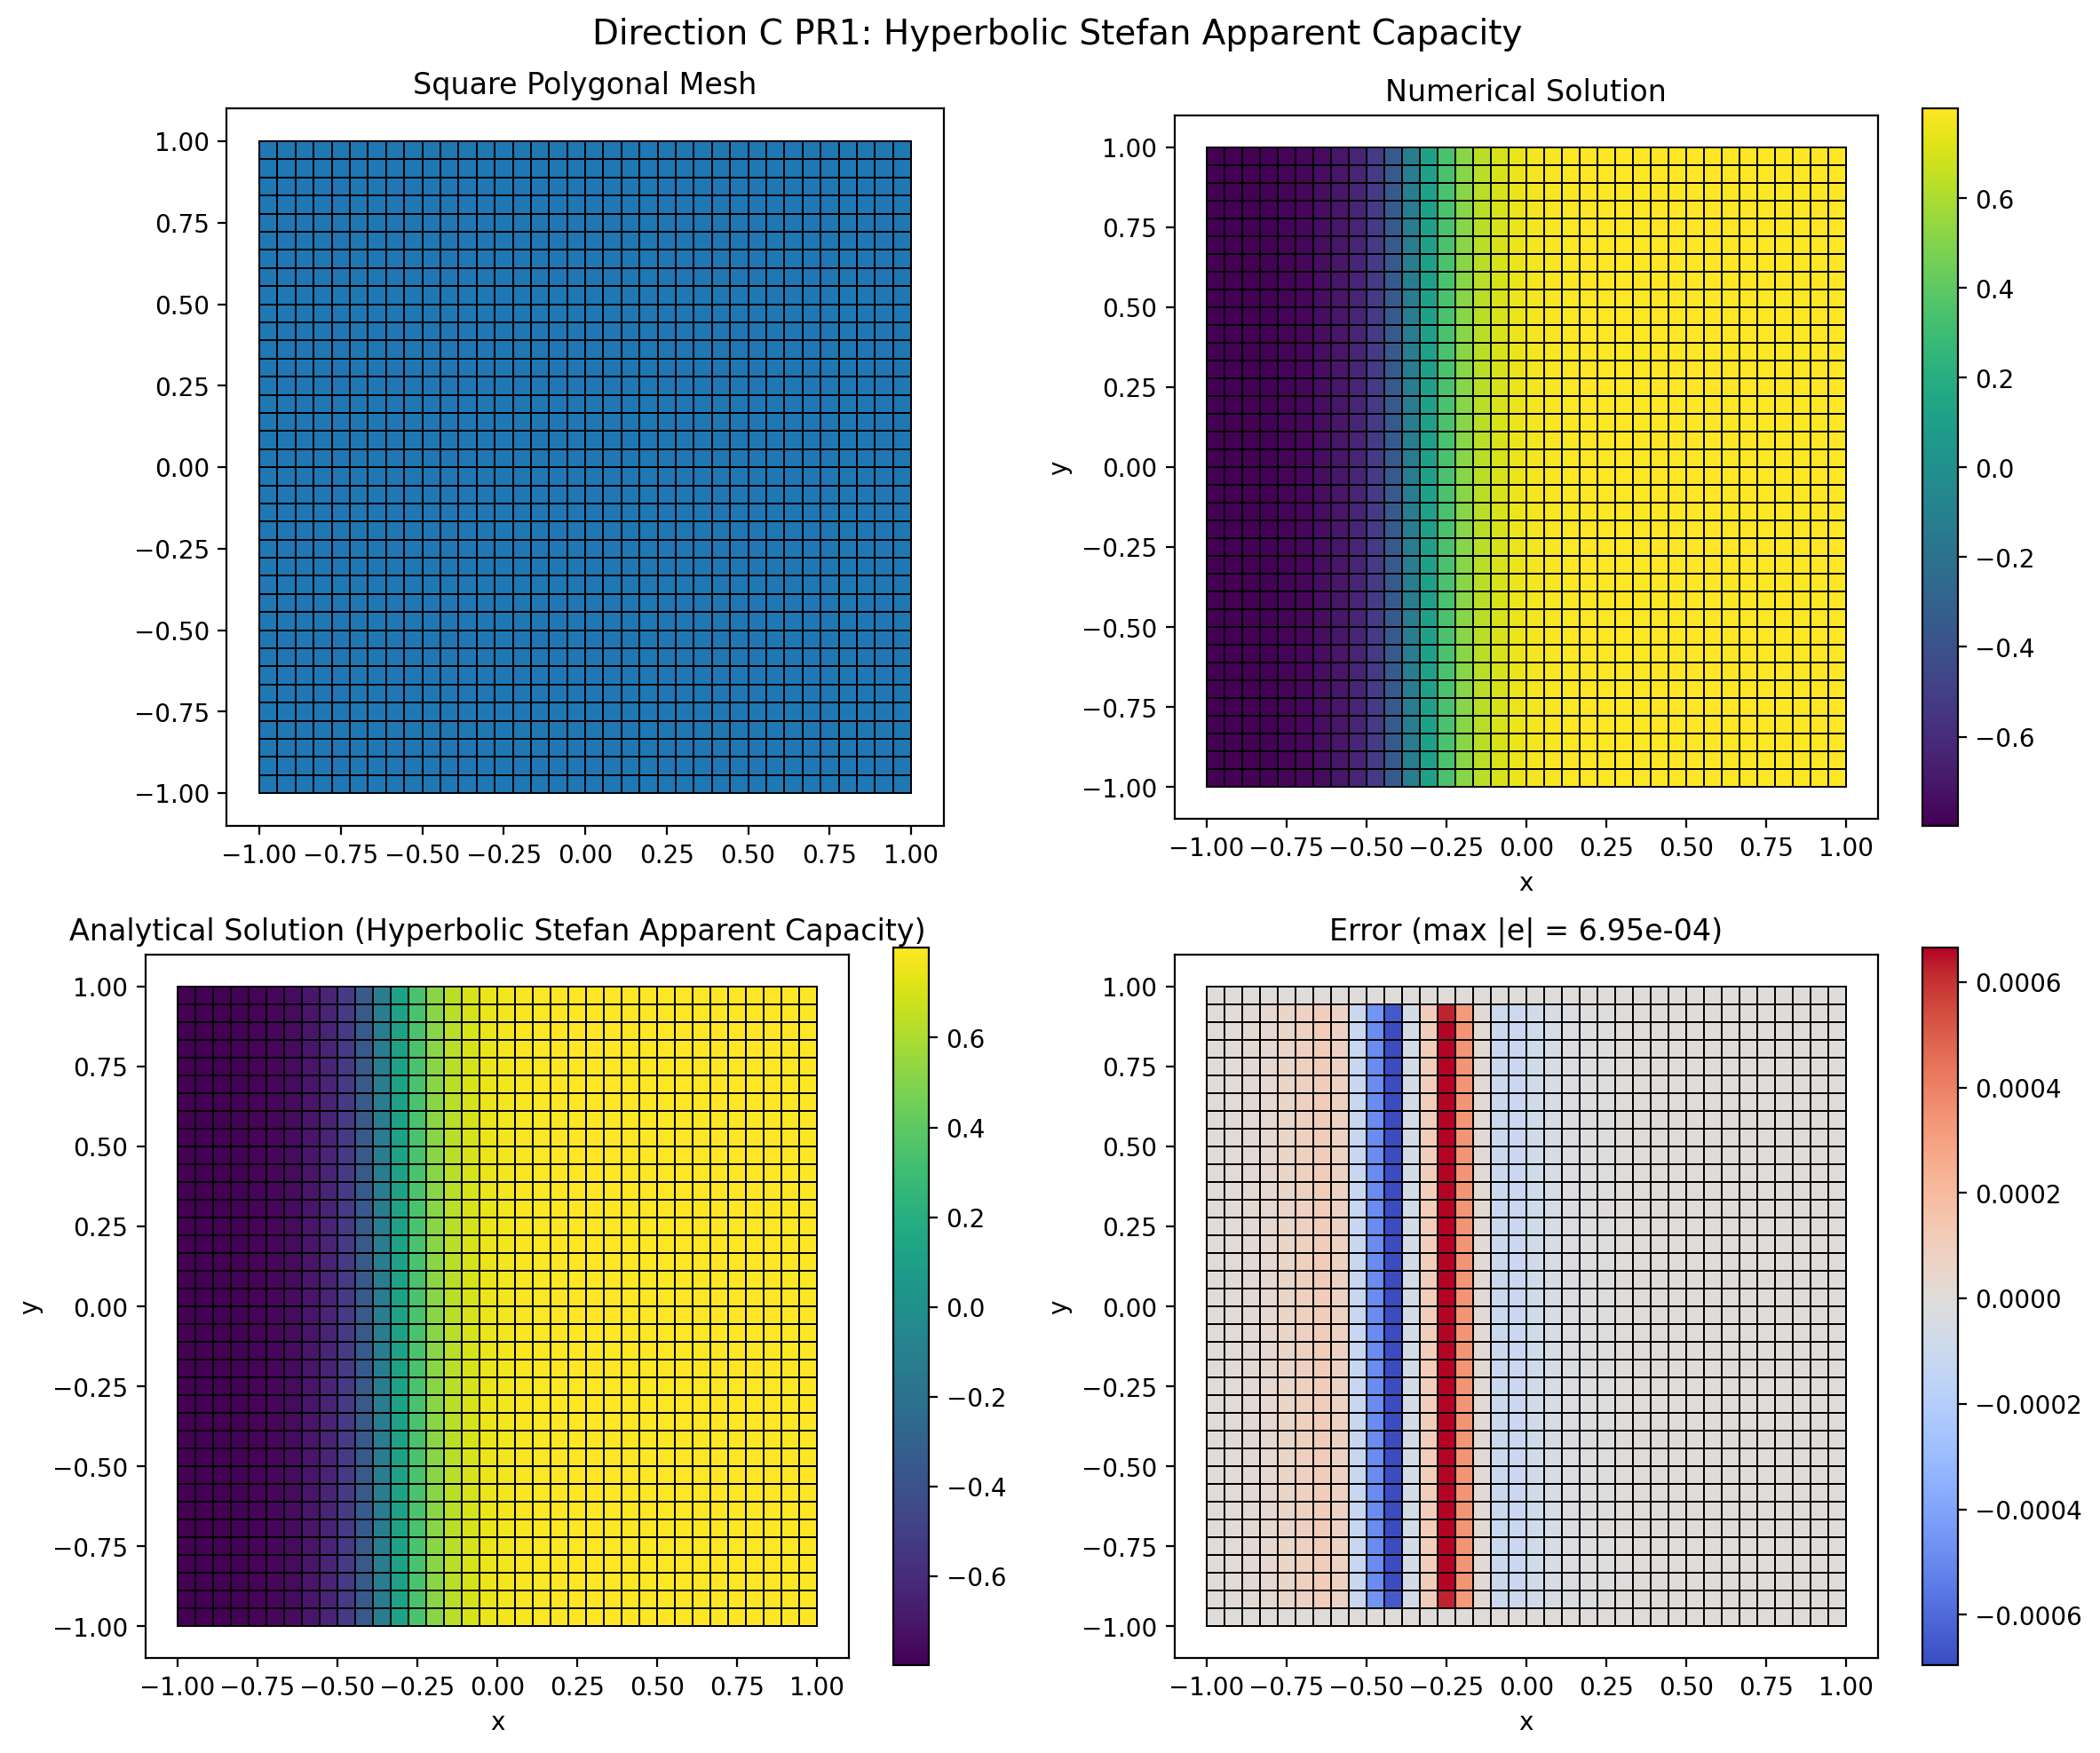
\includegraphics[width=\linewidth]{test_plots/direction_C_nonfourier_phase_change/hyperbolic_stefan_apparent_capacity.png}
    \caption{Hyperbolic Stefan verification.}
  \end{subfigure}
  \hfill
  \begin{subfigure}{0.49\linewidth}
    \centering
    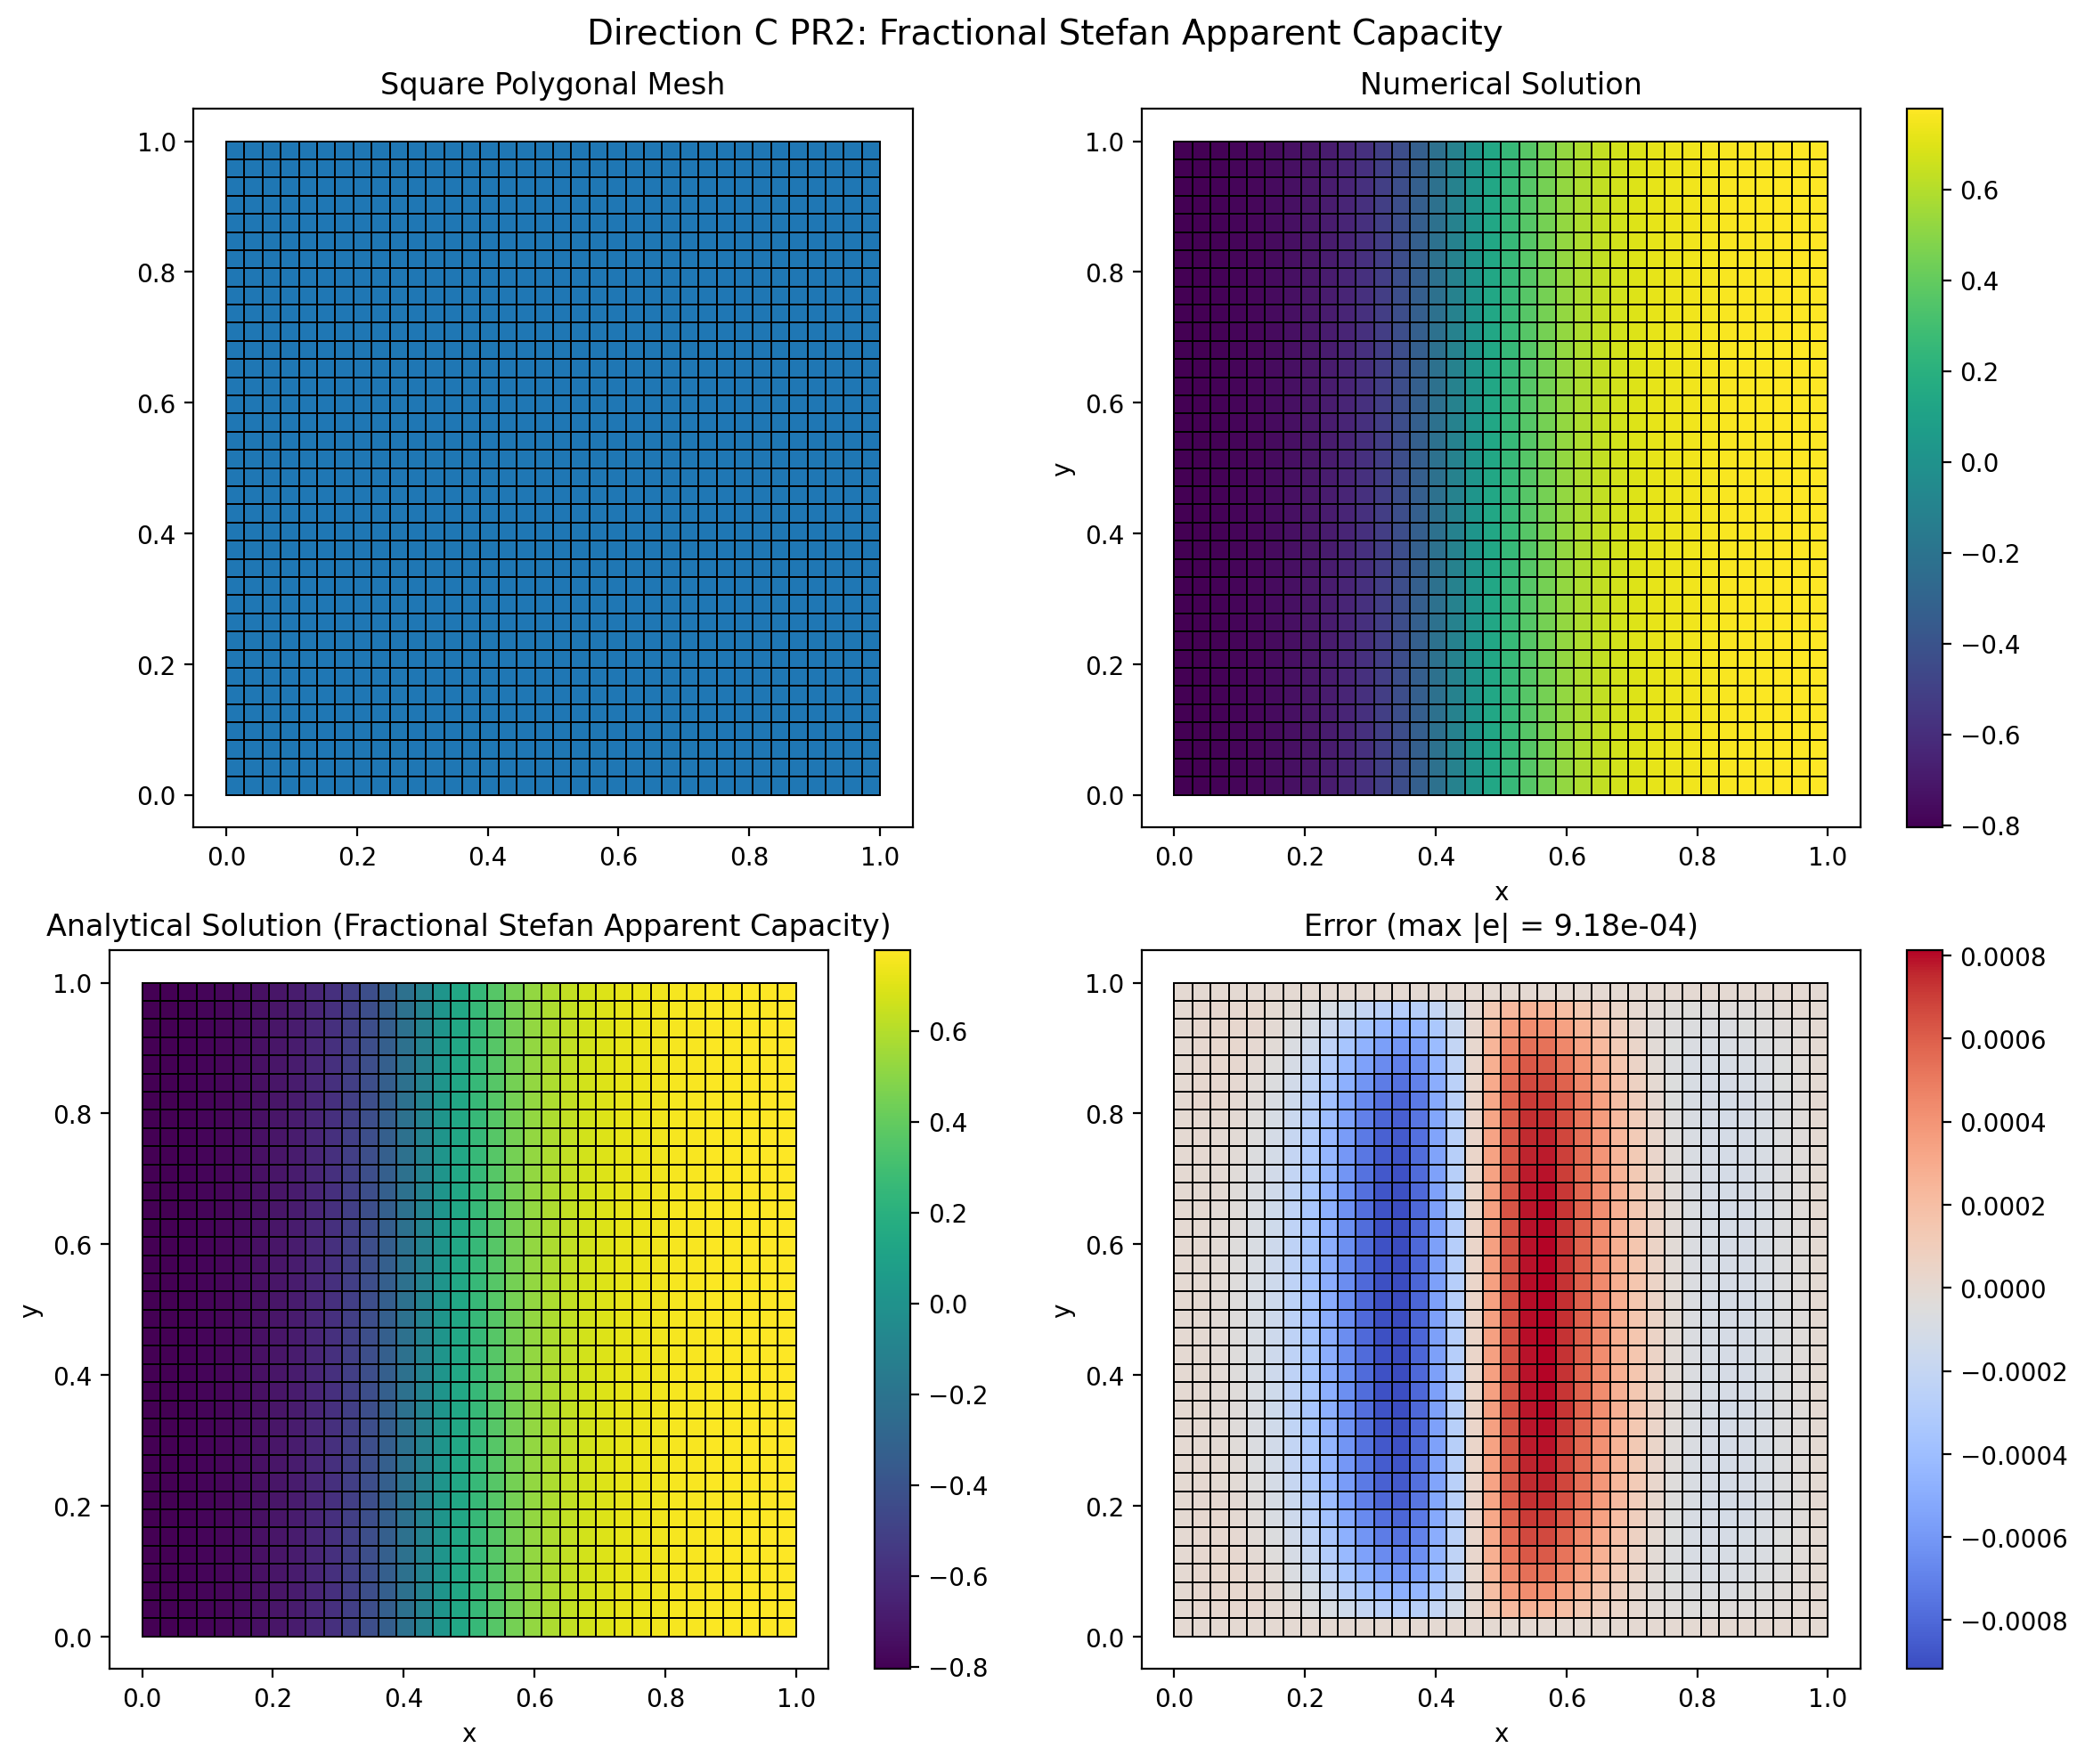
\includegraphics[width=\linewidth]{test_plots/direction_C_nonfourier_phase_change/fractional_stefan_apparent_capacity.png}
    \caption{Fractional Stefan verification.}
  \end{subfigure}
  \caption{Manufactured Direction C verification fields for hyperbolic and fractional apparent-capacity Stefan problems. The left panel uses the Cattaneo relaxation model with a traveling $\tanh$ interface; the right panel uses a Caputo fractional-time model with a smooth moving front. Both figures are generated by the existing Direction C verification workflow and compare the finite-volume field against manufactured exact data.}
\label{fig:direction-c-verification}

\end{figure}

\section{Numerical Implementation}

\subsection{Finite-Volume Semi-Discretization}

Direction C reuses the cell-centered finite-volume geometry and diffusion
operator already used by the verified heat solvers.  After spatial
discretization, the diffusion term has the form
\begin{equation}
  M\,\dot{\bm{T}} + A\bm{T} = \bm{q}
  \label{eq:semi-discrete-heat}
\end{equation}
for a linear Fourier problem, where $M$ is a diagonal cell-area mass matrix,
$A$ is the finite-volume diffusion matrix, and $\bm{q}$ contains source and
boundary contributions.  With phase change, the mass factor is replaced by a
temperature-dependent effective capacity:
\begin{equation}
  M_{\mathrm{eff}}(\bm{T})
  =
  \operatorname{diag}\left(|K_i|\,c_{\mathrm{eff}}(T_i)\right),
  \label{eq:effective-mass}
\end{equation}
where $K_i$ is cell $i$ and $|K_i|$ is its area.

\subsection{Hyperbolic Three-Level Update}

The hyperbolic model requires $T_{tt}$.  The implemented time step uses a
three-level update involving $\bm{T}^{n+1}$, $\bm{T}^{n}$, and
$\bm{T}^{n-1}$.  In simplified notation, each Picard iteration solves
\begin{equation}
  \left[
    \frac{\tau}{\Delta t^2}M
    + \frac{1}{2\Delta t}M_{\mathrm{eff}}(\bm{T}^{(k)})
    + A
  \right]\bm{T}^{(k+1)}
  =
  \bm{b}(\bm{T}^{n},\bm{T}^{n-1},\bm{T}^{(k)}).
  \label{eq:hyperbolic-linearized-step}
\end{equation}
The superscript $(k)$ is the nonlinear Picard iteration index.  Boundary
conditions and source terms are included in $\bm{b}$.  The initial
$\bm{T}^{-1}$ state is built from the supplied initial rate and the PDE-implied
initial acceleration.

\subsection{Fractional L1 Update}

For the fractional model, the L1 approximation represents the Caputo derivative
as a weighted sum of previous increments:
\begin{equation}
  \DtCaputo{\beta}{T}(t_{n+1})
  \approx
  \frac{\Delta t^{-\beta}}{\Gamma(2-\beta)}
  \sum_{j=0}^{n} a_j
  \left(T^{n+1-j}-T^{n-j}\right),
  \qquad
  a_j = (j+1)^{1-\beta}-j^{1-\beta}.
  \label{eq:l1-scheme}
\end{equation}
The new state appears in the $j=0$ term, while older increments form the
history.  The short-memory option keeps only the most recent history terms,
which reduces cost when long simulation times are more important than exact
long-tail memory.

\subsection{Nonlinear Reporting and Energy Audits}

Every nonlinear phase-change solve records iteration counts, failed-step
indices, normalized update residuals, apparent-capacity extrema, relaxation
parameters, and Anderson depth.  For phase-change applications, the enthalpy
audit is
\begin{equation}
  r_E(t)
  =
  \left[H_\Omega(t)-H_\Omega(0)\right]
  -
  \left[E_{\mathrm{in}}(t)-E_{\mathrm{out}}(t)\right],
  \label{eq:energy-audit}
\end{equation}
with
\begin{equation}
  H_\Omega(t) = \sum_i |K_i|\,H(T_i(t)).
  \label{eq:domain-enthalpy}
\end{equation}
The residual $r_E$ is a conservation diagnostic.  For prescribed flux or source
studies, $E_{\mathrm{in}}$ is computed from the known input.  For Dirichlet
cooling studies, the current implementation reports the inferred extracted
energy from the enthalpy loss; explicit boundary-flux reconstruction remains a
useful future refinement.

\section{Expansion Studies}

The expansion-study plots isolate three scientific issues: finite-speed
relaxation, fractional memory, and latent-heat stiffness.

\begin{figure}[t]
  \centering
  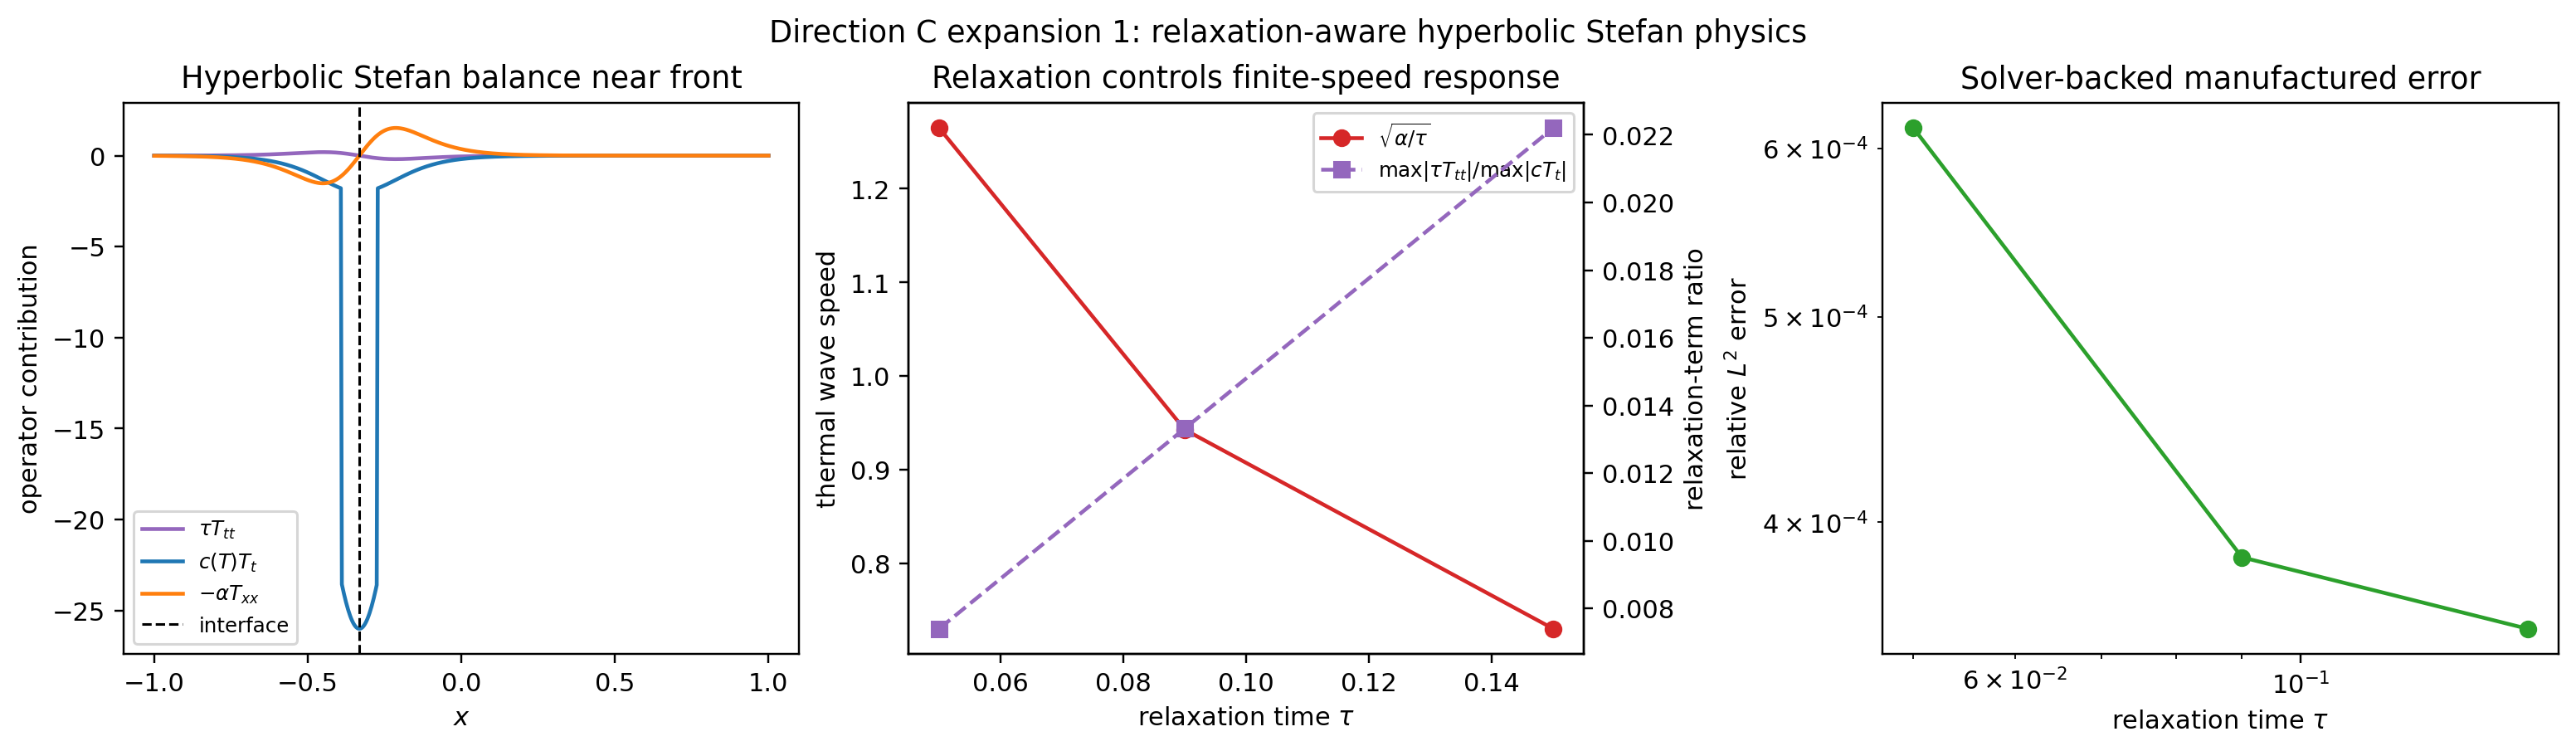
\includegraphics[width=\linewidth]{test_plots/direction_C_nonfourier_phase_change/expansion_studies/hyperbolic_relaxation_balance.png}
  \caption{Relaxation-aware hyperbolic Stefan diagnostics. The figure summarizes how the Cattaneo relaxation time $\tau$ changes the relative balance of wave, storage, and diffusion terms, and records solver-backed manufactured errors and convergence metadata across stable relaxation-time values.}
\label{fig:direction-c-relaxation-balance}

\end{figure}

\begin{figure}[t]
  \centering
  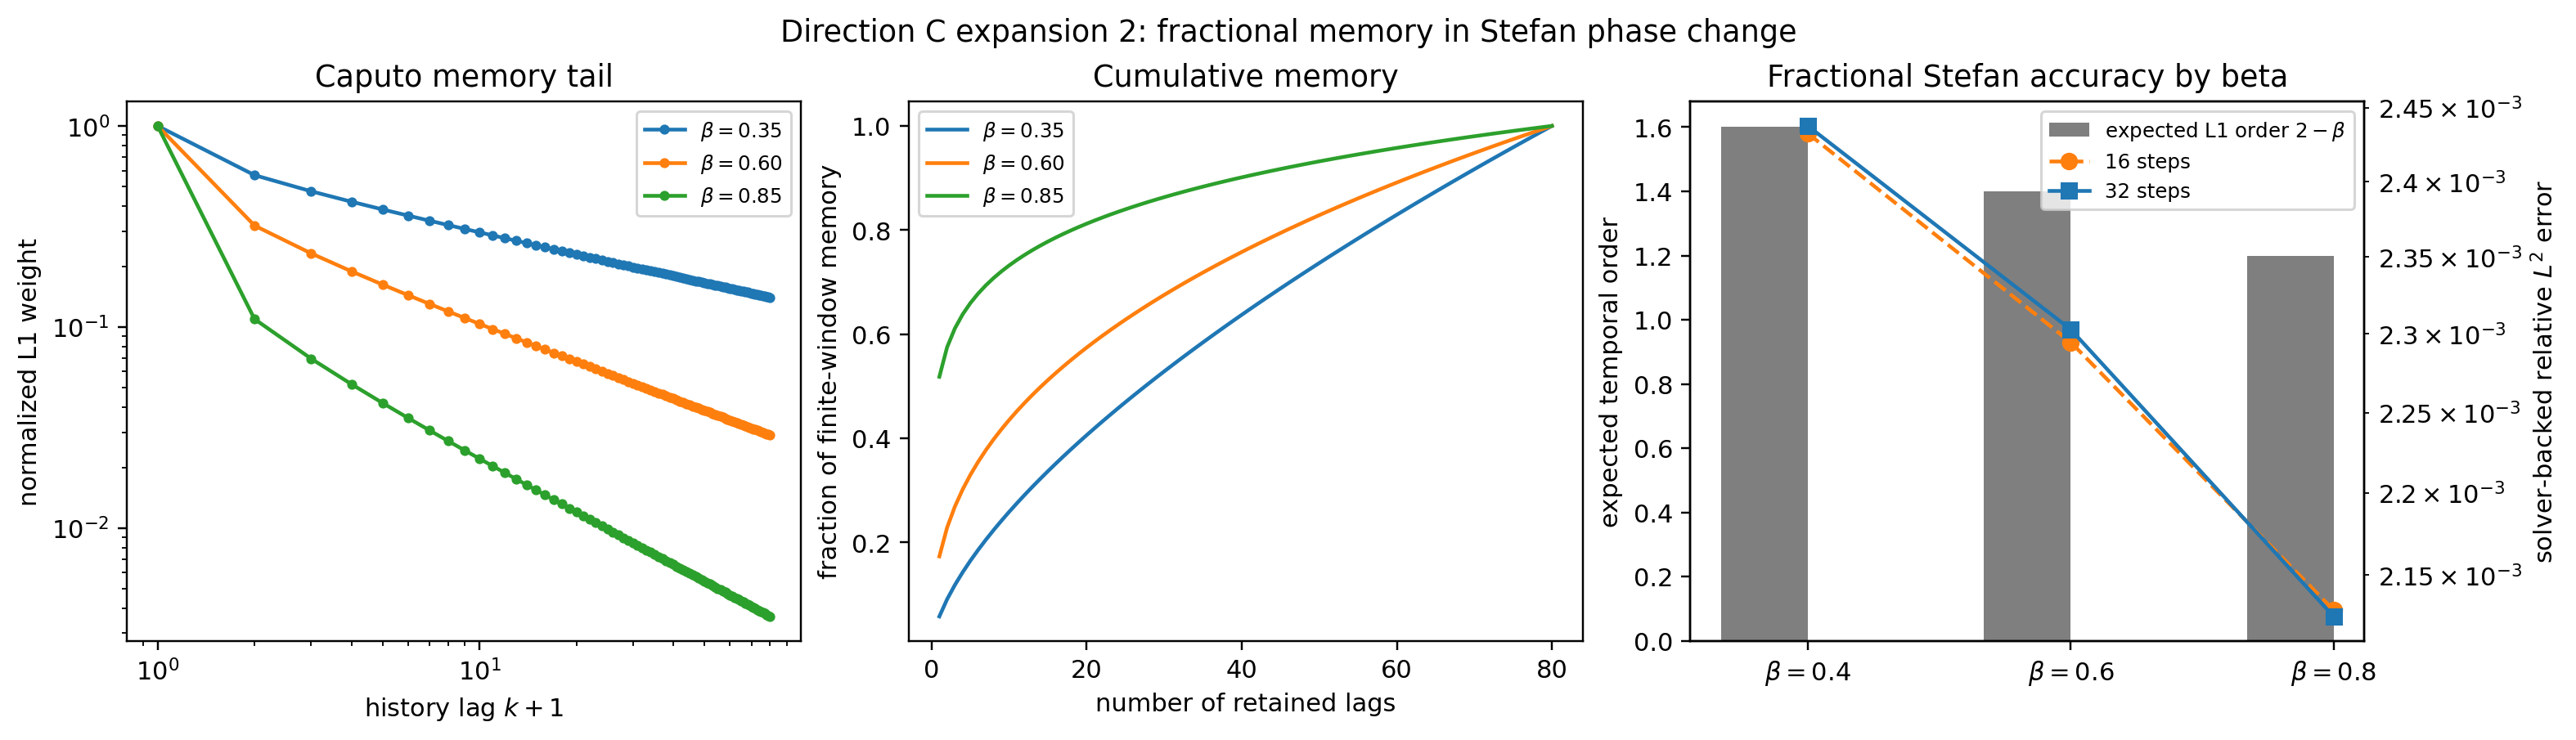
\includegraphics[width=\linewidth]{test_plots/direction_C_nonfourier_phase_change/expansion_studies/fractional_memory_convergence.png}
  \caption{Fractional-memory Stefan diagnostics. The plot shows how the Caputo/L1 history weights retain past thermal states, how observed temporal order tracks the expected $2-\beta$ behavior, and how short-memory truncation trades accuracy for reduced history cost.}
\label{fig:direction-c-fractional-memory}

\end{figure}

\begin{figure}[t]
  \centering
  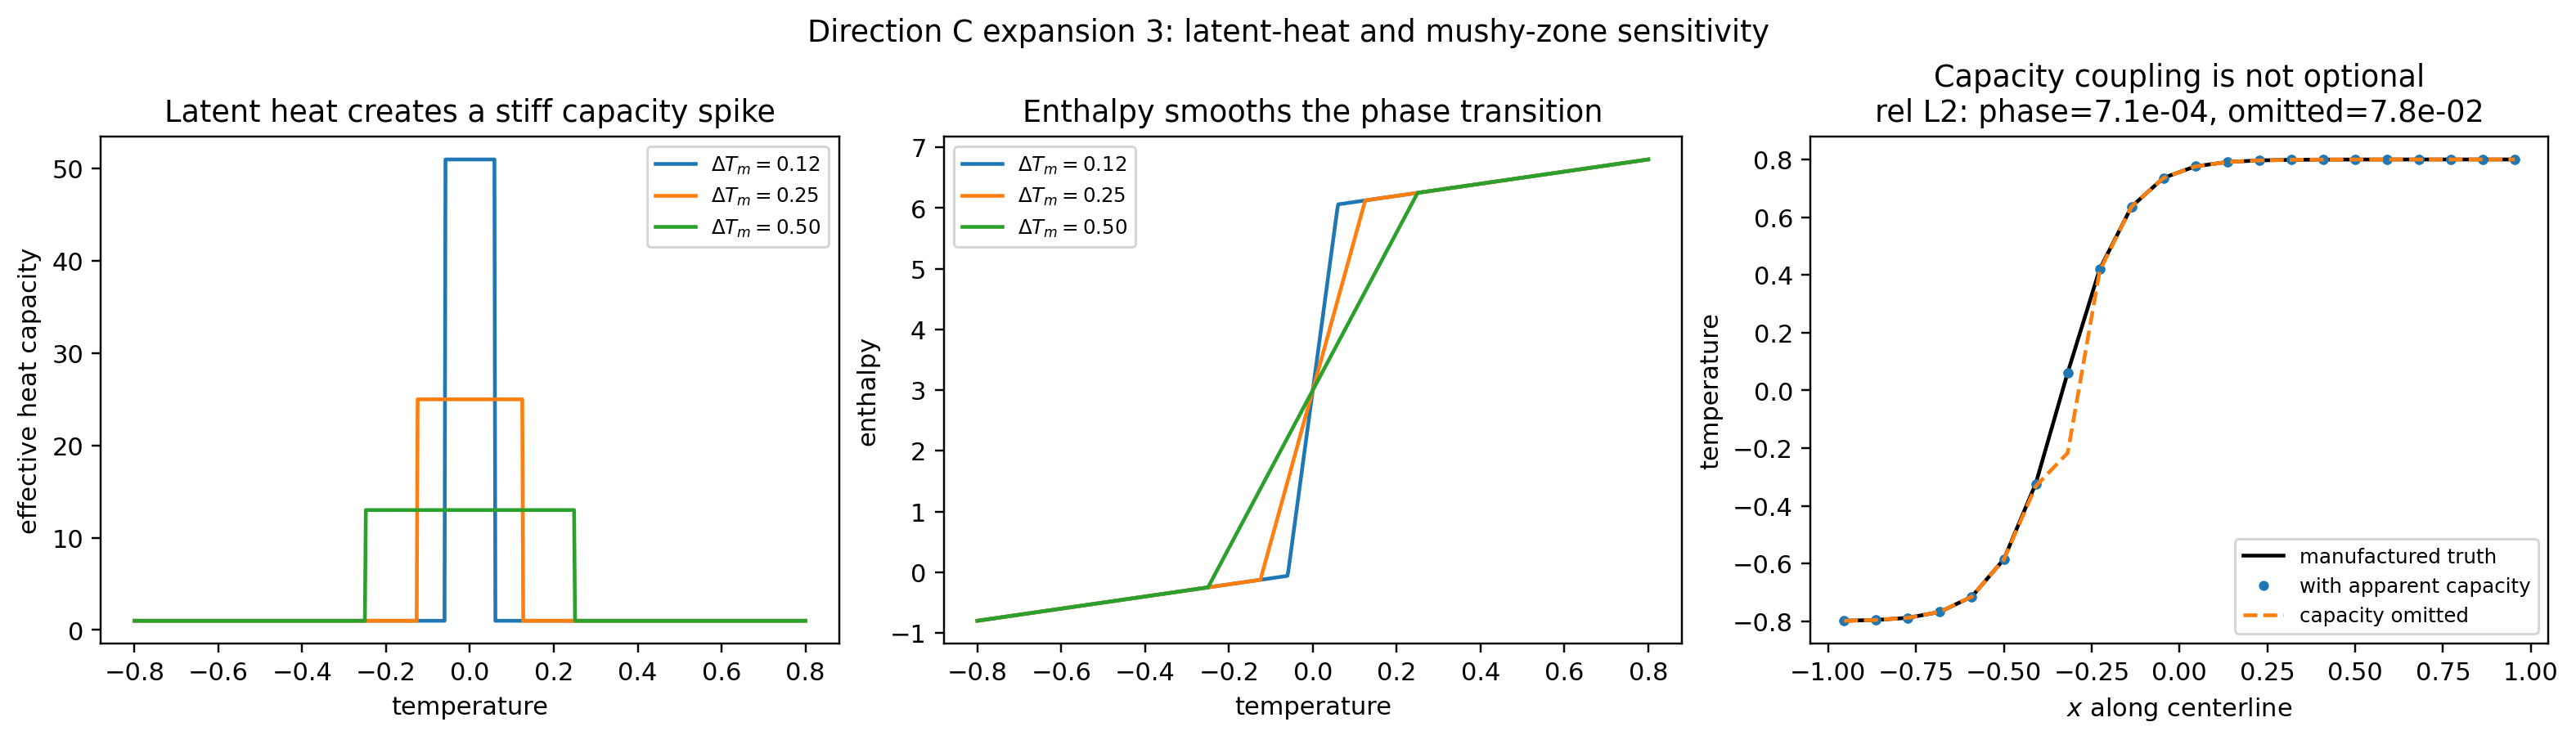
\includegraphics[width=\linewidth]{test_plots/direction_C_nonfourier_phase_change/expansion_studies/mushy_zone_capacity_coupling.png}
  \caption{Latent-heat and mushy-zone stiffness diagnostics. Apparent heat capacity replaces a sharp latent-heat jump with a finite temperature interval, but narrowing that interval creates a large capacity spike that directly affects nonlinear convergence and interface dynamics.}
\label{fig:direction-c-mushy-capacity}

\end{figure}

\section{Application Studies}

The application runners provide physically interpretable two-dimensional
scenarios beyond manufactured verification.  They use the same solver and
diagnostic interfaces but different forcing and boundary conditions:
\begin{description}[leftmargin=3.2cm,style=nextline]
  \item[Pulsed laser melting]
  A boundary heat-flux pulse melts a cold slab.  The runner tracks melt-front
  advance, liquid fraction, mushy thickness, injected energy, and energy
  closure.
  \item[Cryosurgery freezing]
  A cold Dirichlet probe freezes a warm domain.  The runner reports freezing
  margin, frozen fraction, minimum temperature, and inferred enthalpy removal.
  \item[Moving scan melt pool]
  A moving Gaussian volumetric source creates an additive-manufacturing-like
  melt track.  The runner reports melt-pool length and width, source energy,
  liquid fraction, and mushy thickness.
  \item[Dual-pulse remelting]
  Two separated flux pulses probe latent-heat retention and remelting between
  pulses.
  \item[Rapid solidification quench]
  A hot liquid slab cools against cold boundaries, showing liquid-fraction
  collapse and solid-fraction growth.
  \item[Buried hot inclusion relaxation]
  A localized hot inclusion cools and refreezes inside a colder matrix, giving
  a compact test of internal phase-change relaxation.
\end{description}

\begin{figure}[p]
  \centering
  \begin{subfigure}{0.32\linewidth}
    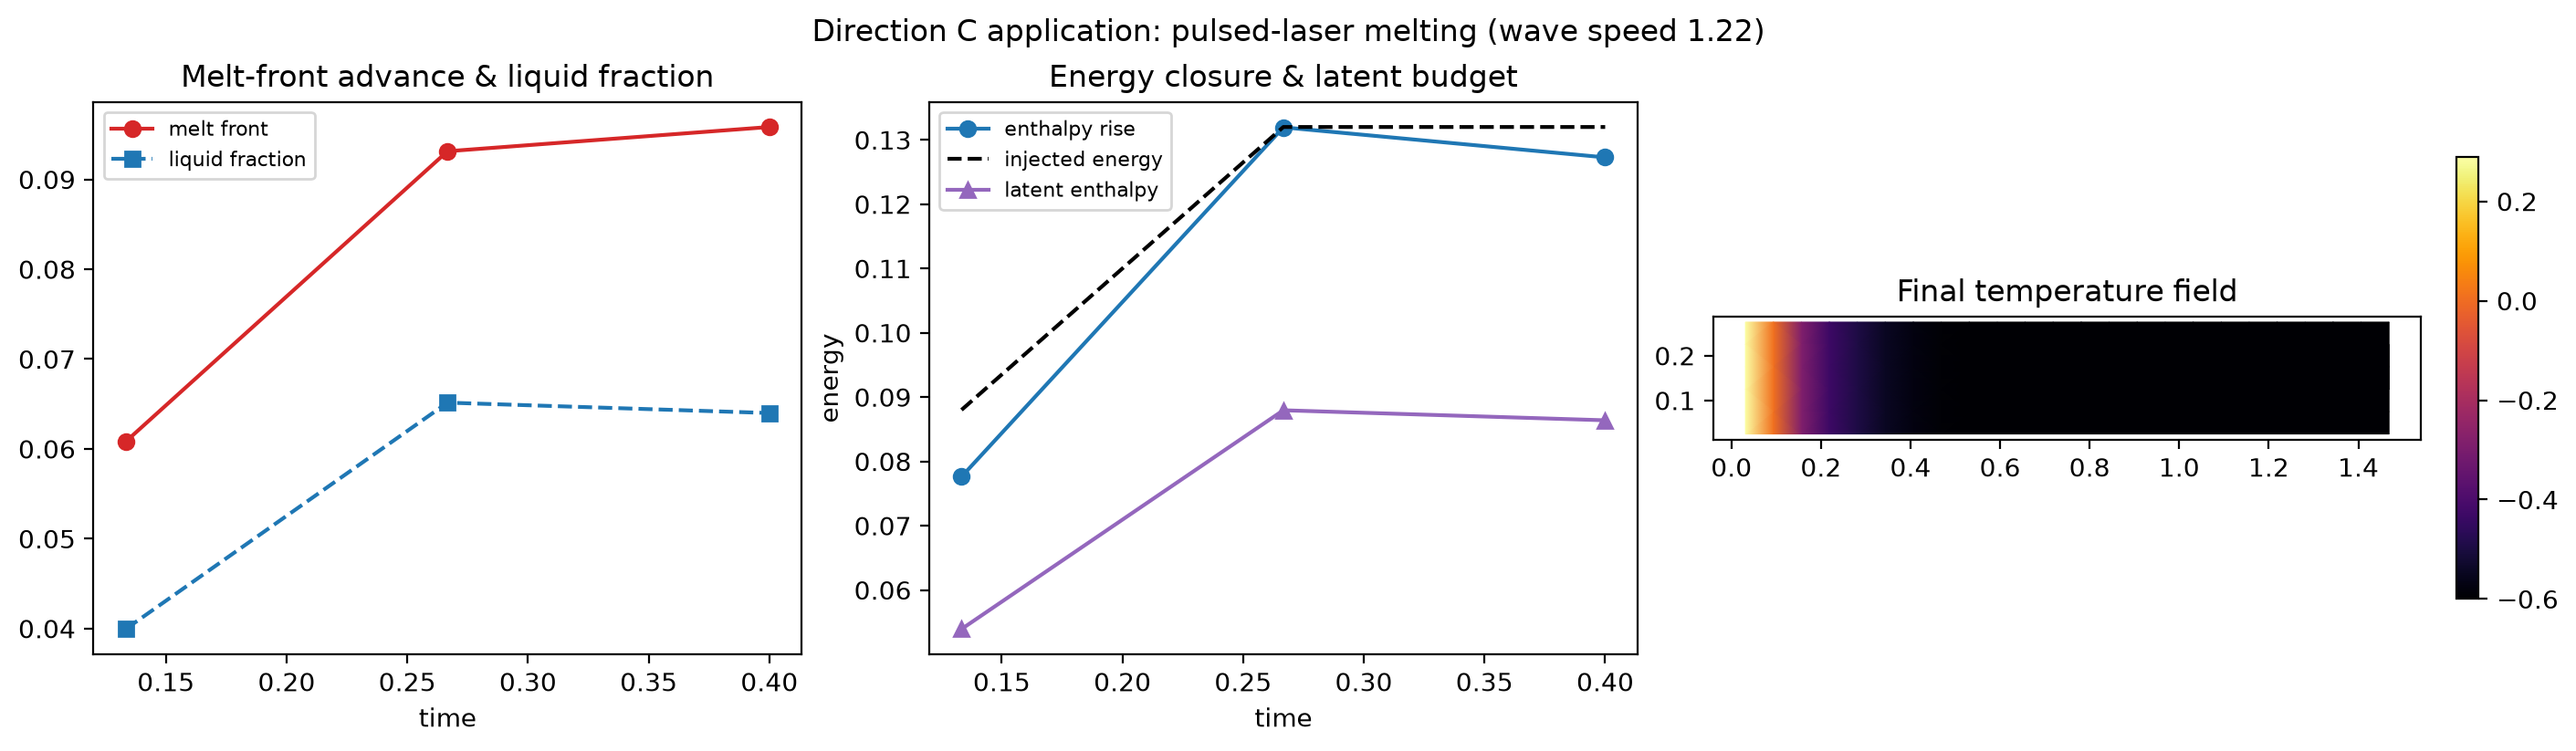
\includegraphics[width=\linewidth]{test_plots/direction_C_nonfourier_phase_change/applications/pulsed_laser_melting.png}
    \caption{Laser melting.}
  \end{subfigure}
  \begin{subfigure}{0.32\linewidth}
    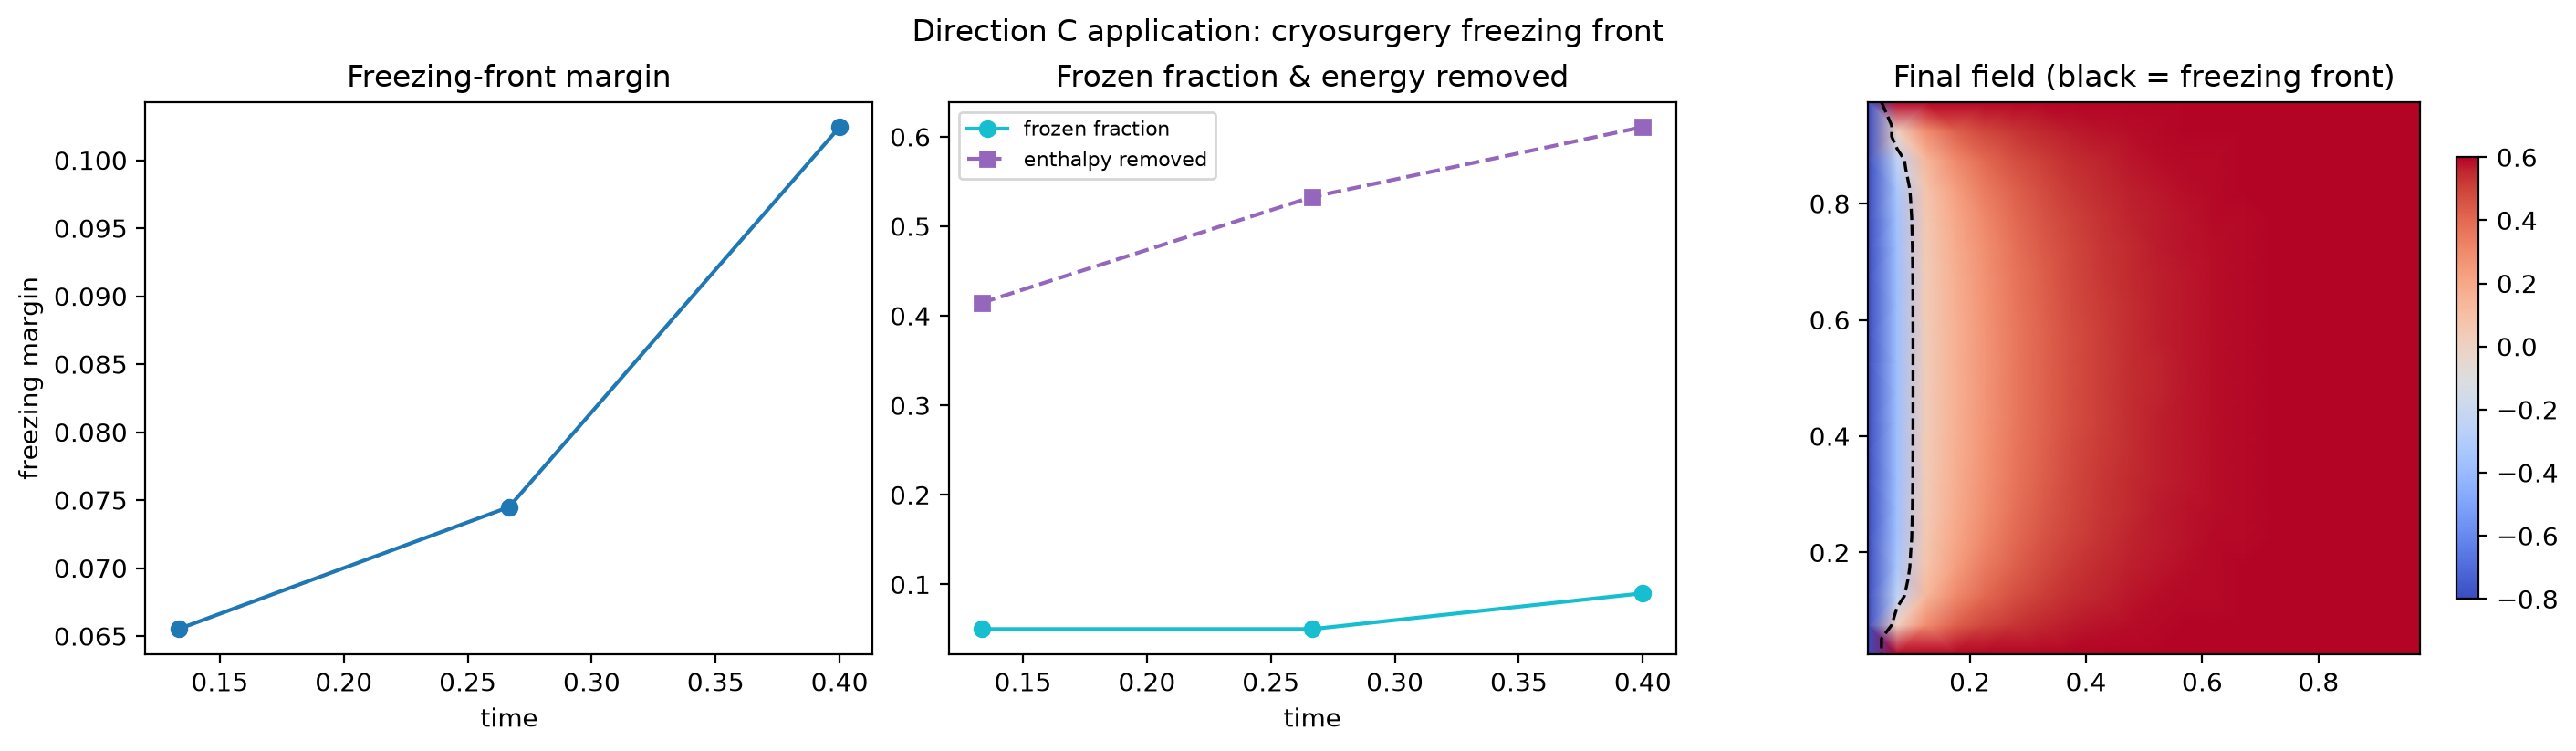
\includegraphics[width=\linewidth]{test_plots/direction_C_nonfourier_phase_change/applications/cryosurgery_freezing.png}
    \caption{Cryosurgery.}
  \end{subfigure}
  \begin{subfigure}{0.32\linewidth}
    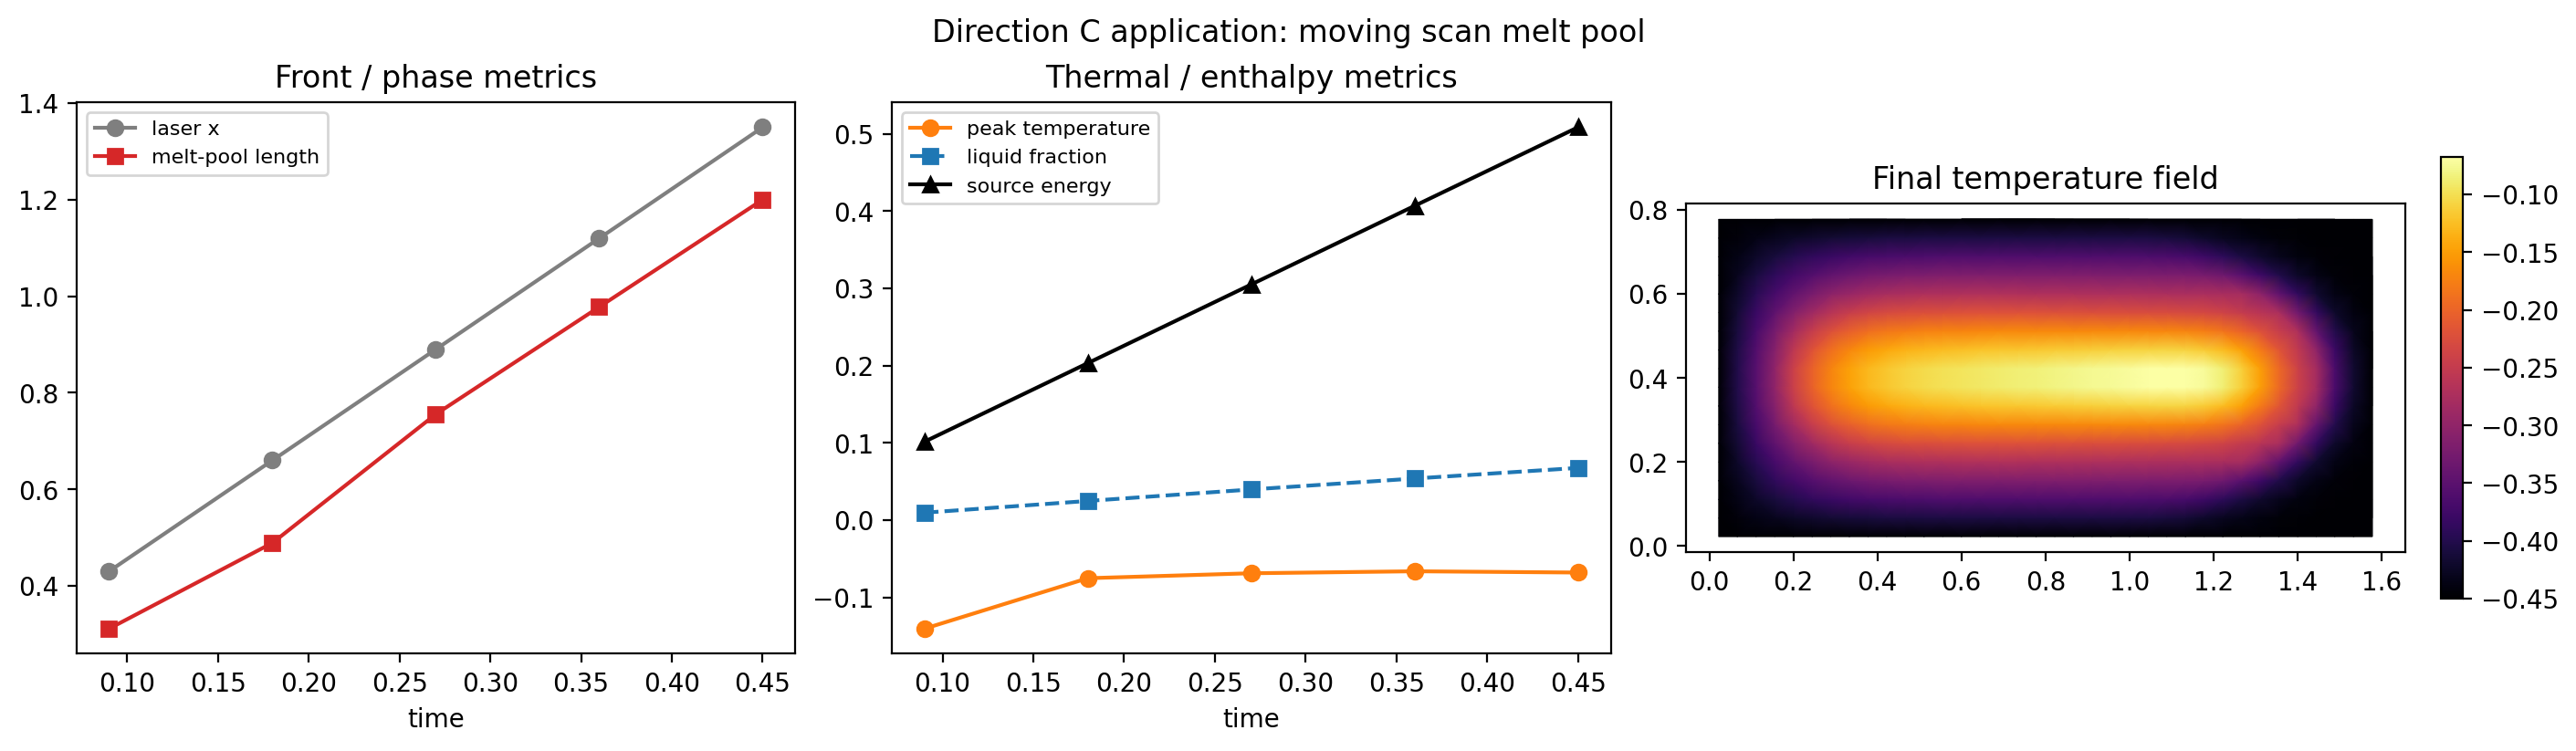
\includegraphics[width=\linewidth]{test_plots/direction_C_nonfourier_phase_change/applications/moving_scan_melt_pool.png}
    \caption{Scan melt pool.}
  \end{subfigure}

  \vspace{0.6em}
  \begin{subfigure}{0.32\linewidth}
    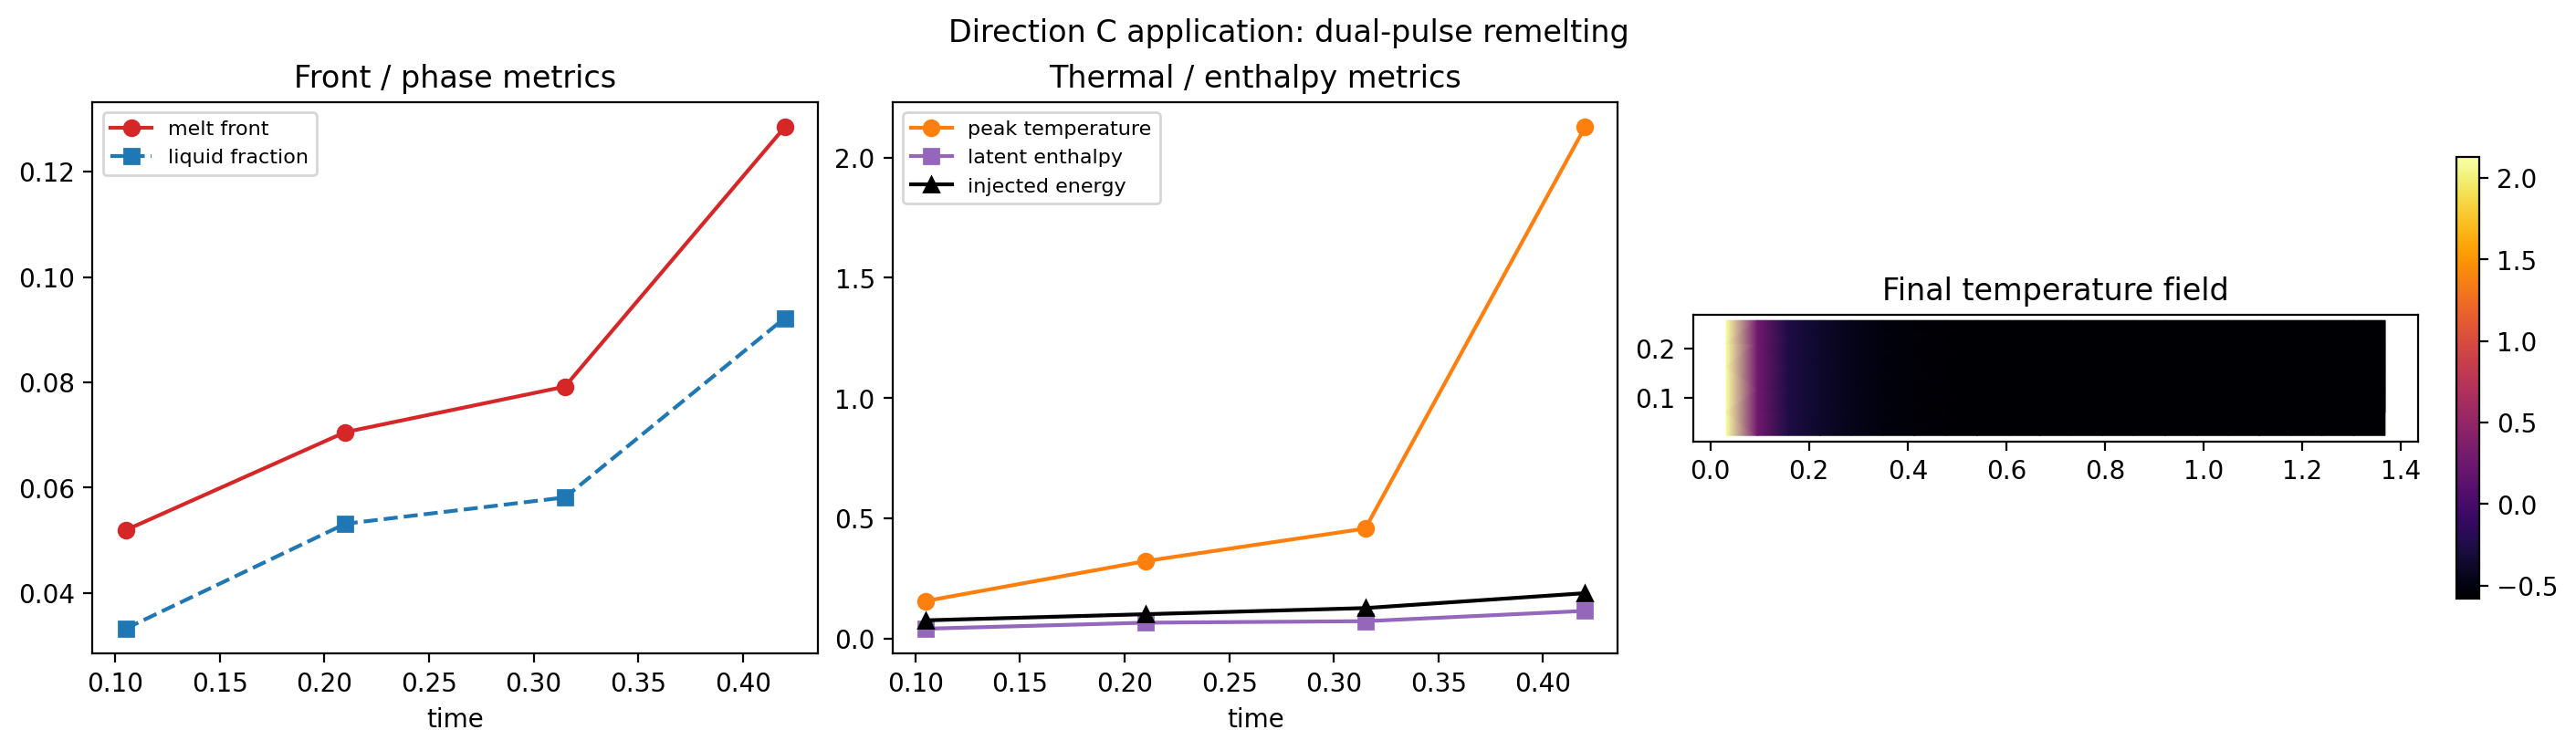
\includegraphics[width=\linewidth]{test_plots/direction_C_nonfourier_phase_change/applications/dual_pulse_remelting.png}
    \caption{Dual-pulse remelting.}
  \end{subfigure}
  \begin{subfigure}{0.32\linewidth}
    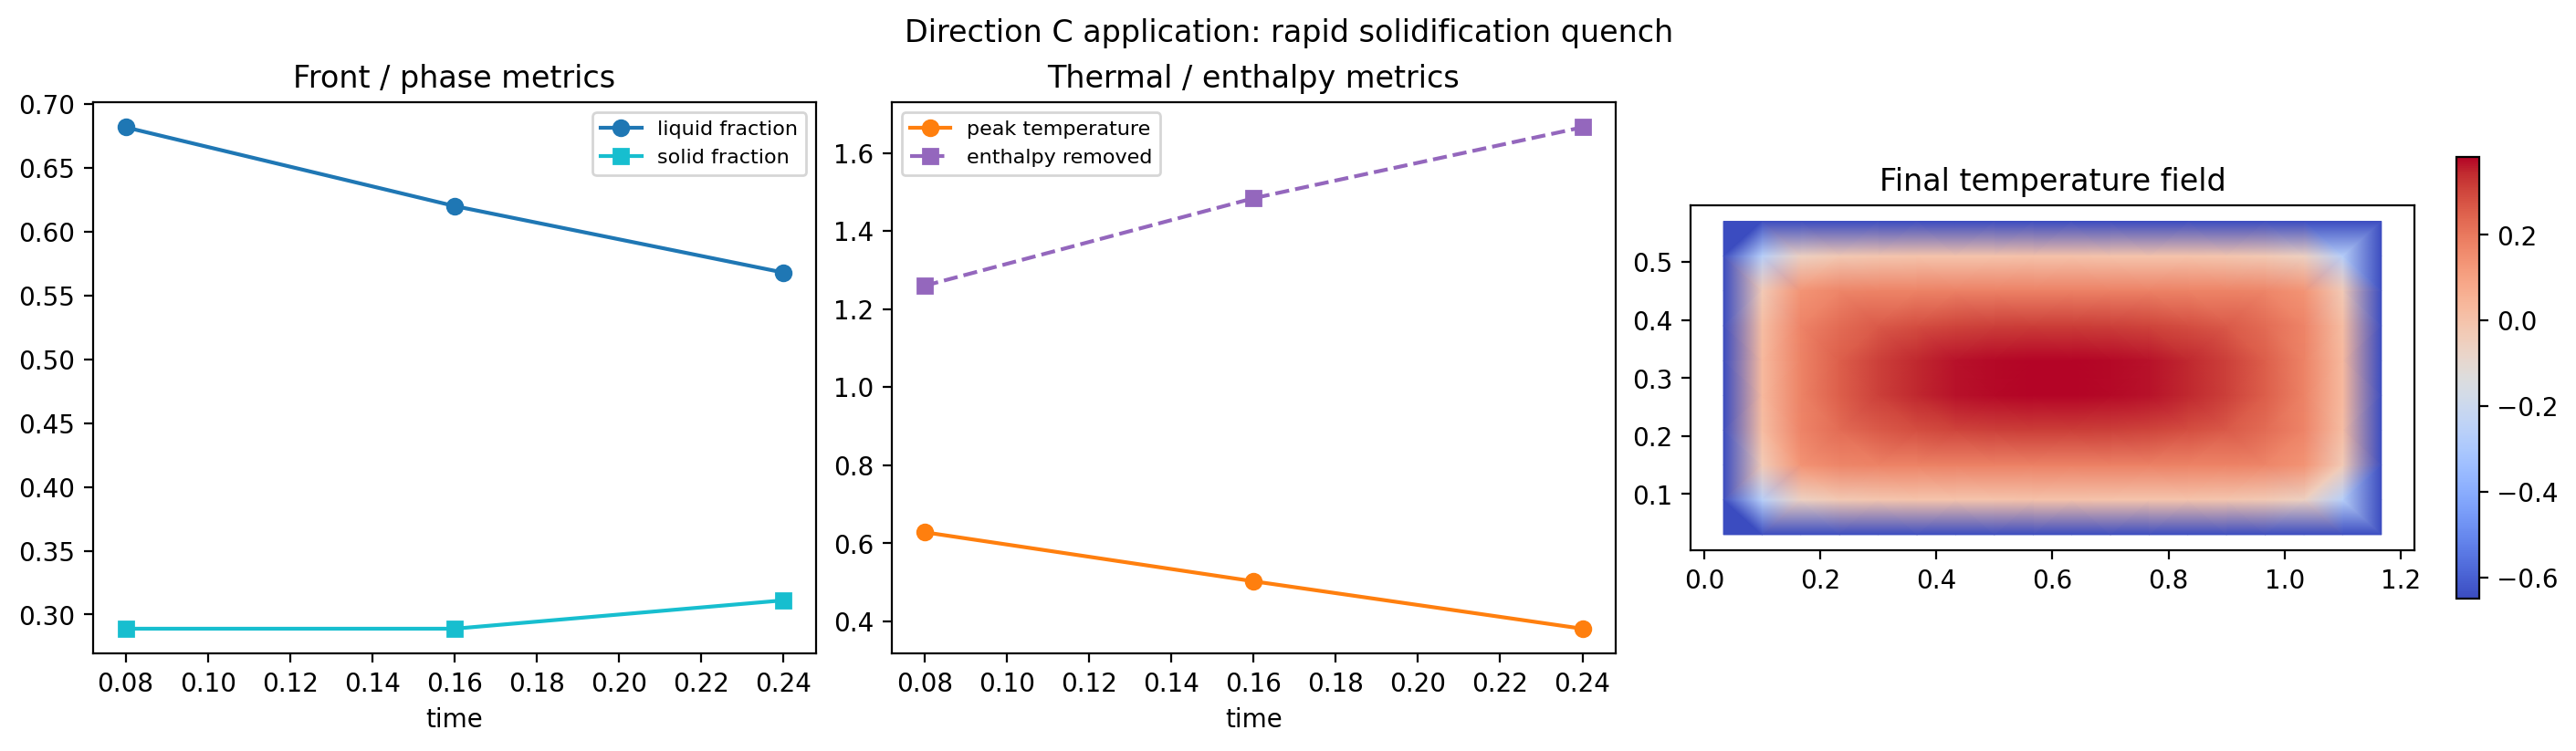
\includegraphics[width=\linewidth]{test_plots/direction_C_nonfourier_phase_change/applications/rapid_solidification_quench.png}
    \caption{Rapid quench.}
  \end{subfigure}
  \begin{subfigure}{0.32\linewidth}
    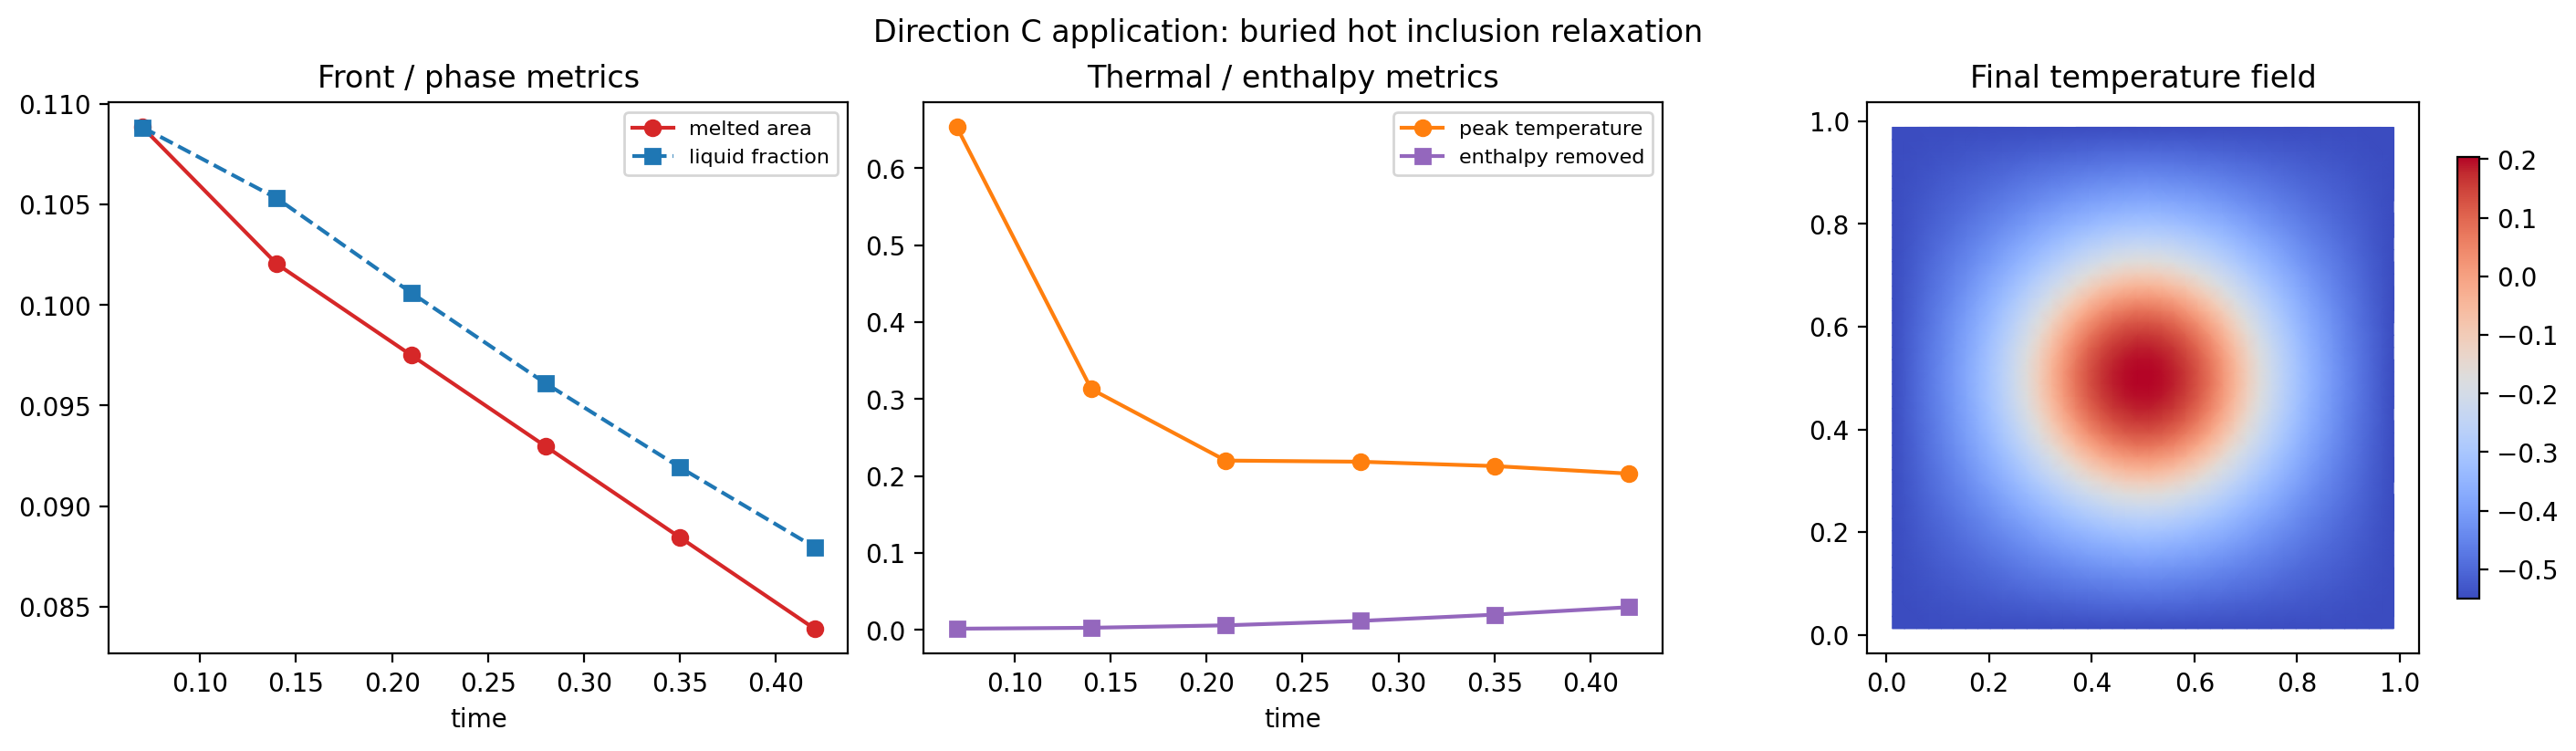
\includegraphics[width=\linewidth]{test_plots/direction_C_nonfourier_phase_change/applications/buried_hot_inclusion_relaxation.png}
    \caption{Buried inclusion.}
  \end{subfigure}
  \caption{Representative Direction C application studies. Pulsed laser melting, cryosurgery freezing, additive-manufacturing-like scanning, dual-pulse remelting, rapid quenching, and buried-inclusion relaxation exercise the same non-Fourier apparent-capacity machinery under physically distinct forcing and boundary conditions.}
\label{fig:direction-c-application-gallery}

\end{figure}

\begin{figure}[p]
  \centering
  \begin{subfigure}{0.49\linewidth}
    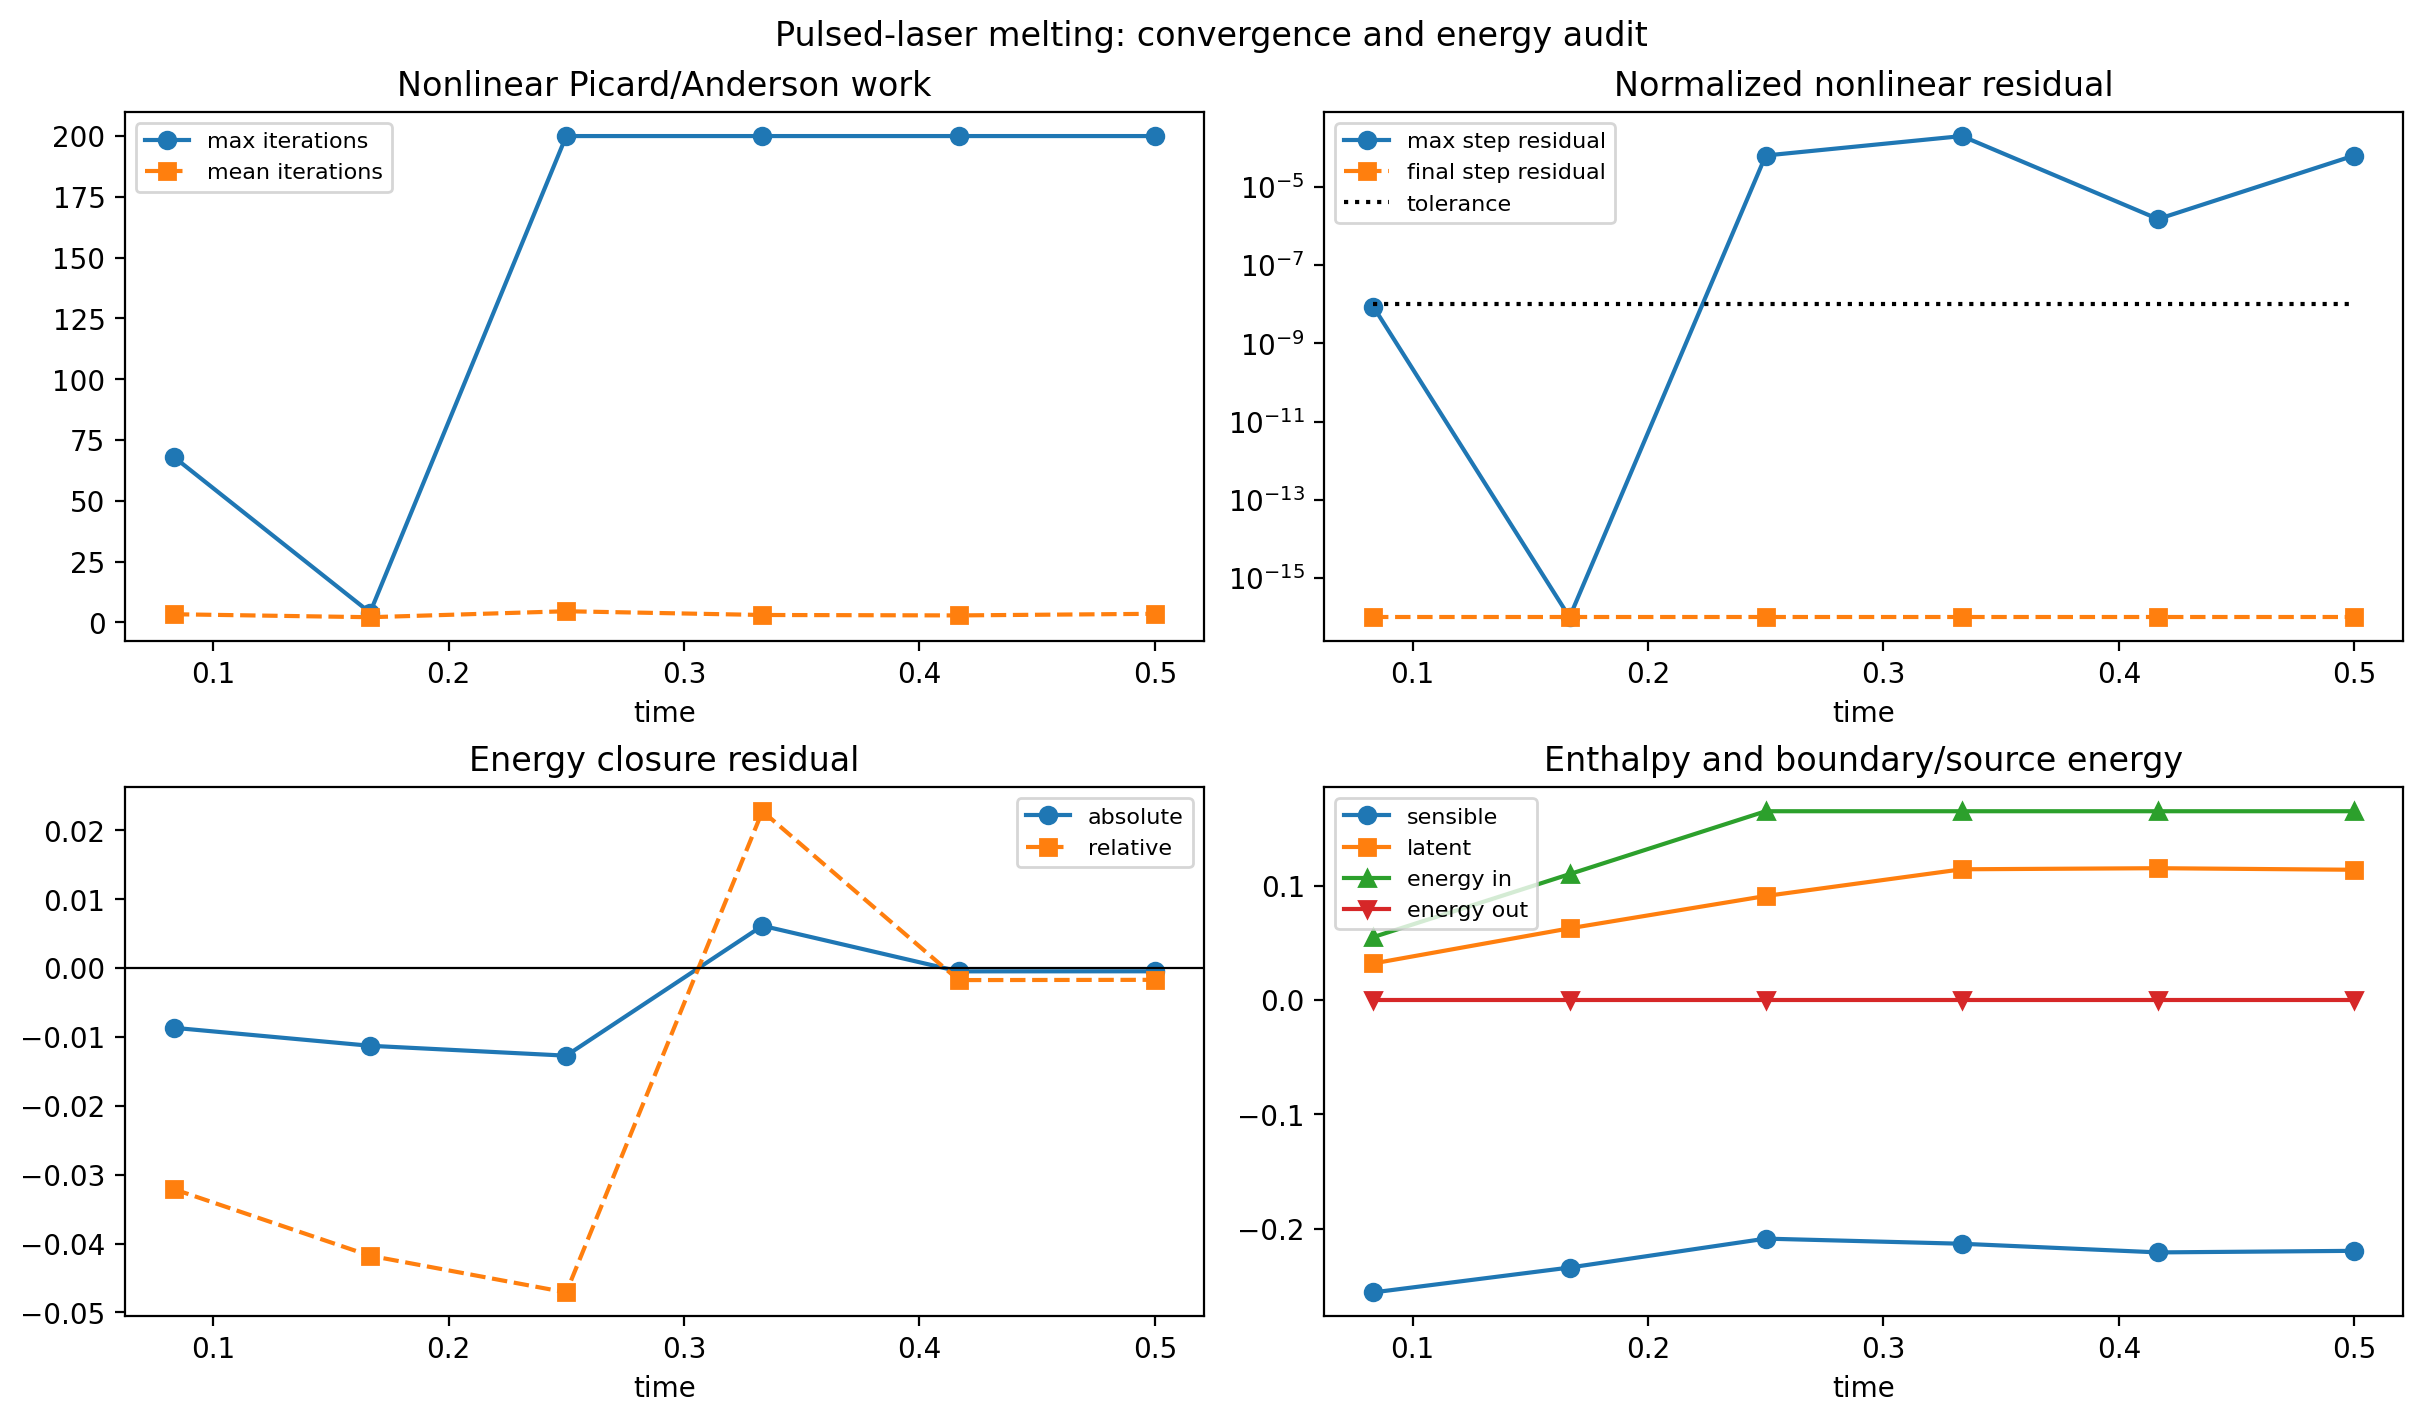
\includegraphics[width=\linewidth]{test_plots/direction_C_nonfourier_phase_change/applications/pulsed_laser_melting_diagnostics.png}
    \caption{Flux-driven laser audit.}
  \end{subfigure}
  \hfill
  \begin{subfigure}{0.49\linewidth}
    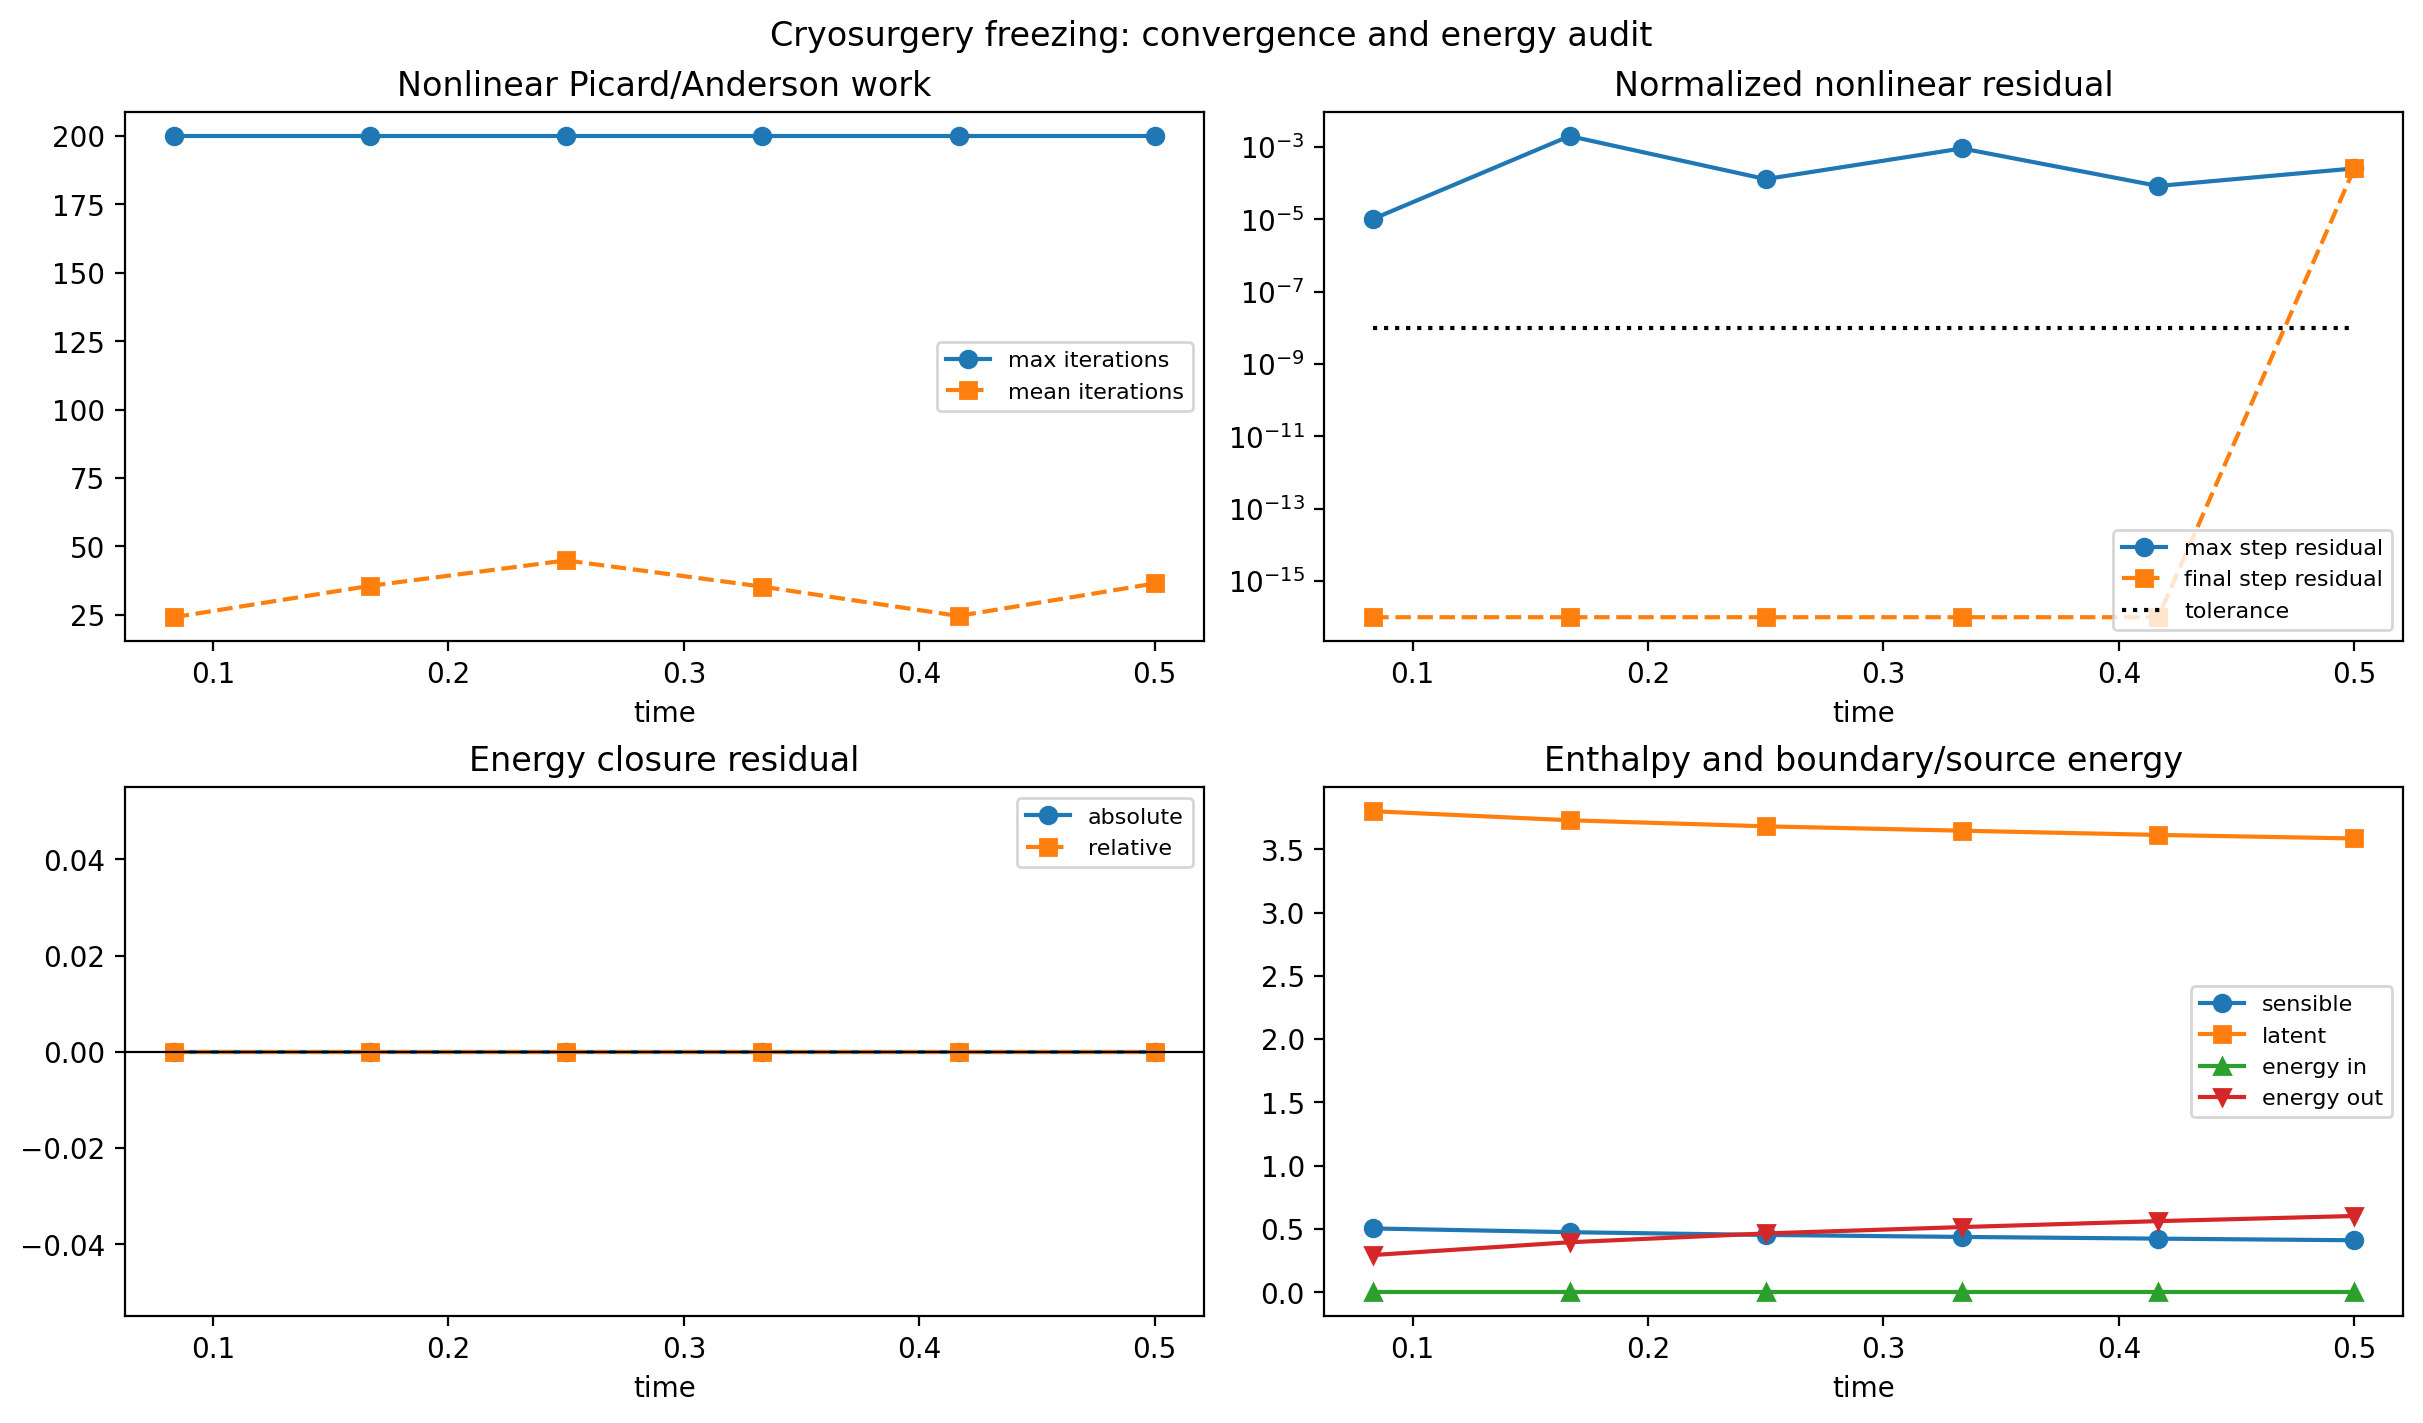
\includegraphics[width=\linewidth]{test_plots/direction_C_nonfourier_phase_change/applications/cryosurgery_freezing_diagnostics.png}
    \caption{Cooling-driven freezing audit.}
  \end{subfigure}
  \caption{Application-level nonlinear and energy diagnostics. The dashboards expose Picard/Anderson iteration counts, normalized nonlinear residuals, apparent-capacity extrema, sensible and latent enthalpy histories, and energy-closure residuals for flux-driven and cooling-driven phase-change scenarios.}
\label{fig:direction-c-diagnostics-gallery}

\end{figure}

\section{Parameter-Sweep Infrastructure}

Direction C's final implementation step is a sparse benchmark matrix rather
than an exhaustive Cartesian product.  The suite sweeps one main axis at a time
around a baseline, then includes one stiff combined hyperbolic case.  The
recorded fields are
\begin{equation}
  \left\{
  \tau,\ \beta,\ L,\ T_l-T_s,\ s,\ n_h,\ n_t,\ \Delta t,\ 
  \norm{T_h-T_{\mathrm{exact}}}_{L^2},\
  \text{iterations},\ \text{failures},\ c_{\mathrm{eff,max}}
  \right\}.
  \label{eq:sweep-fields}
\end{equation}
Here $n_h$ is a spatial resolution parameter and $n_t$ is the number of time
steps.  The purpose is not to replace a full design-of-experiments campaign,
but to make a compact research dataset that continuously exercises the main
Direction C physics and numerics.

\begin{figure}[t]
  \centering
  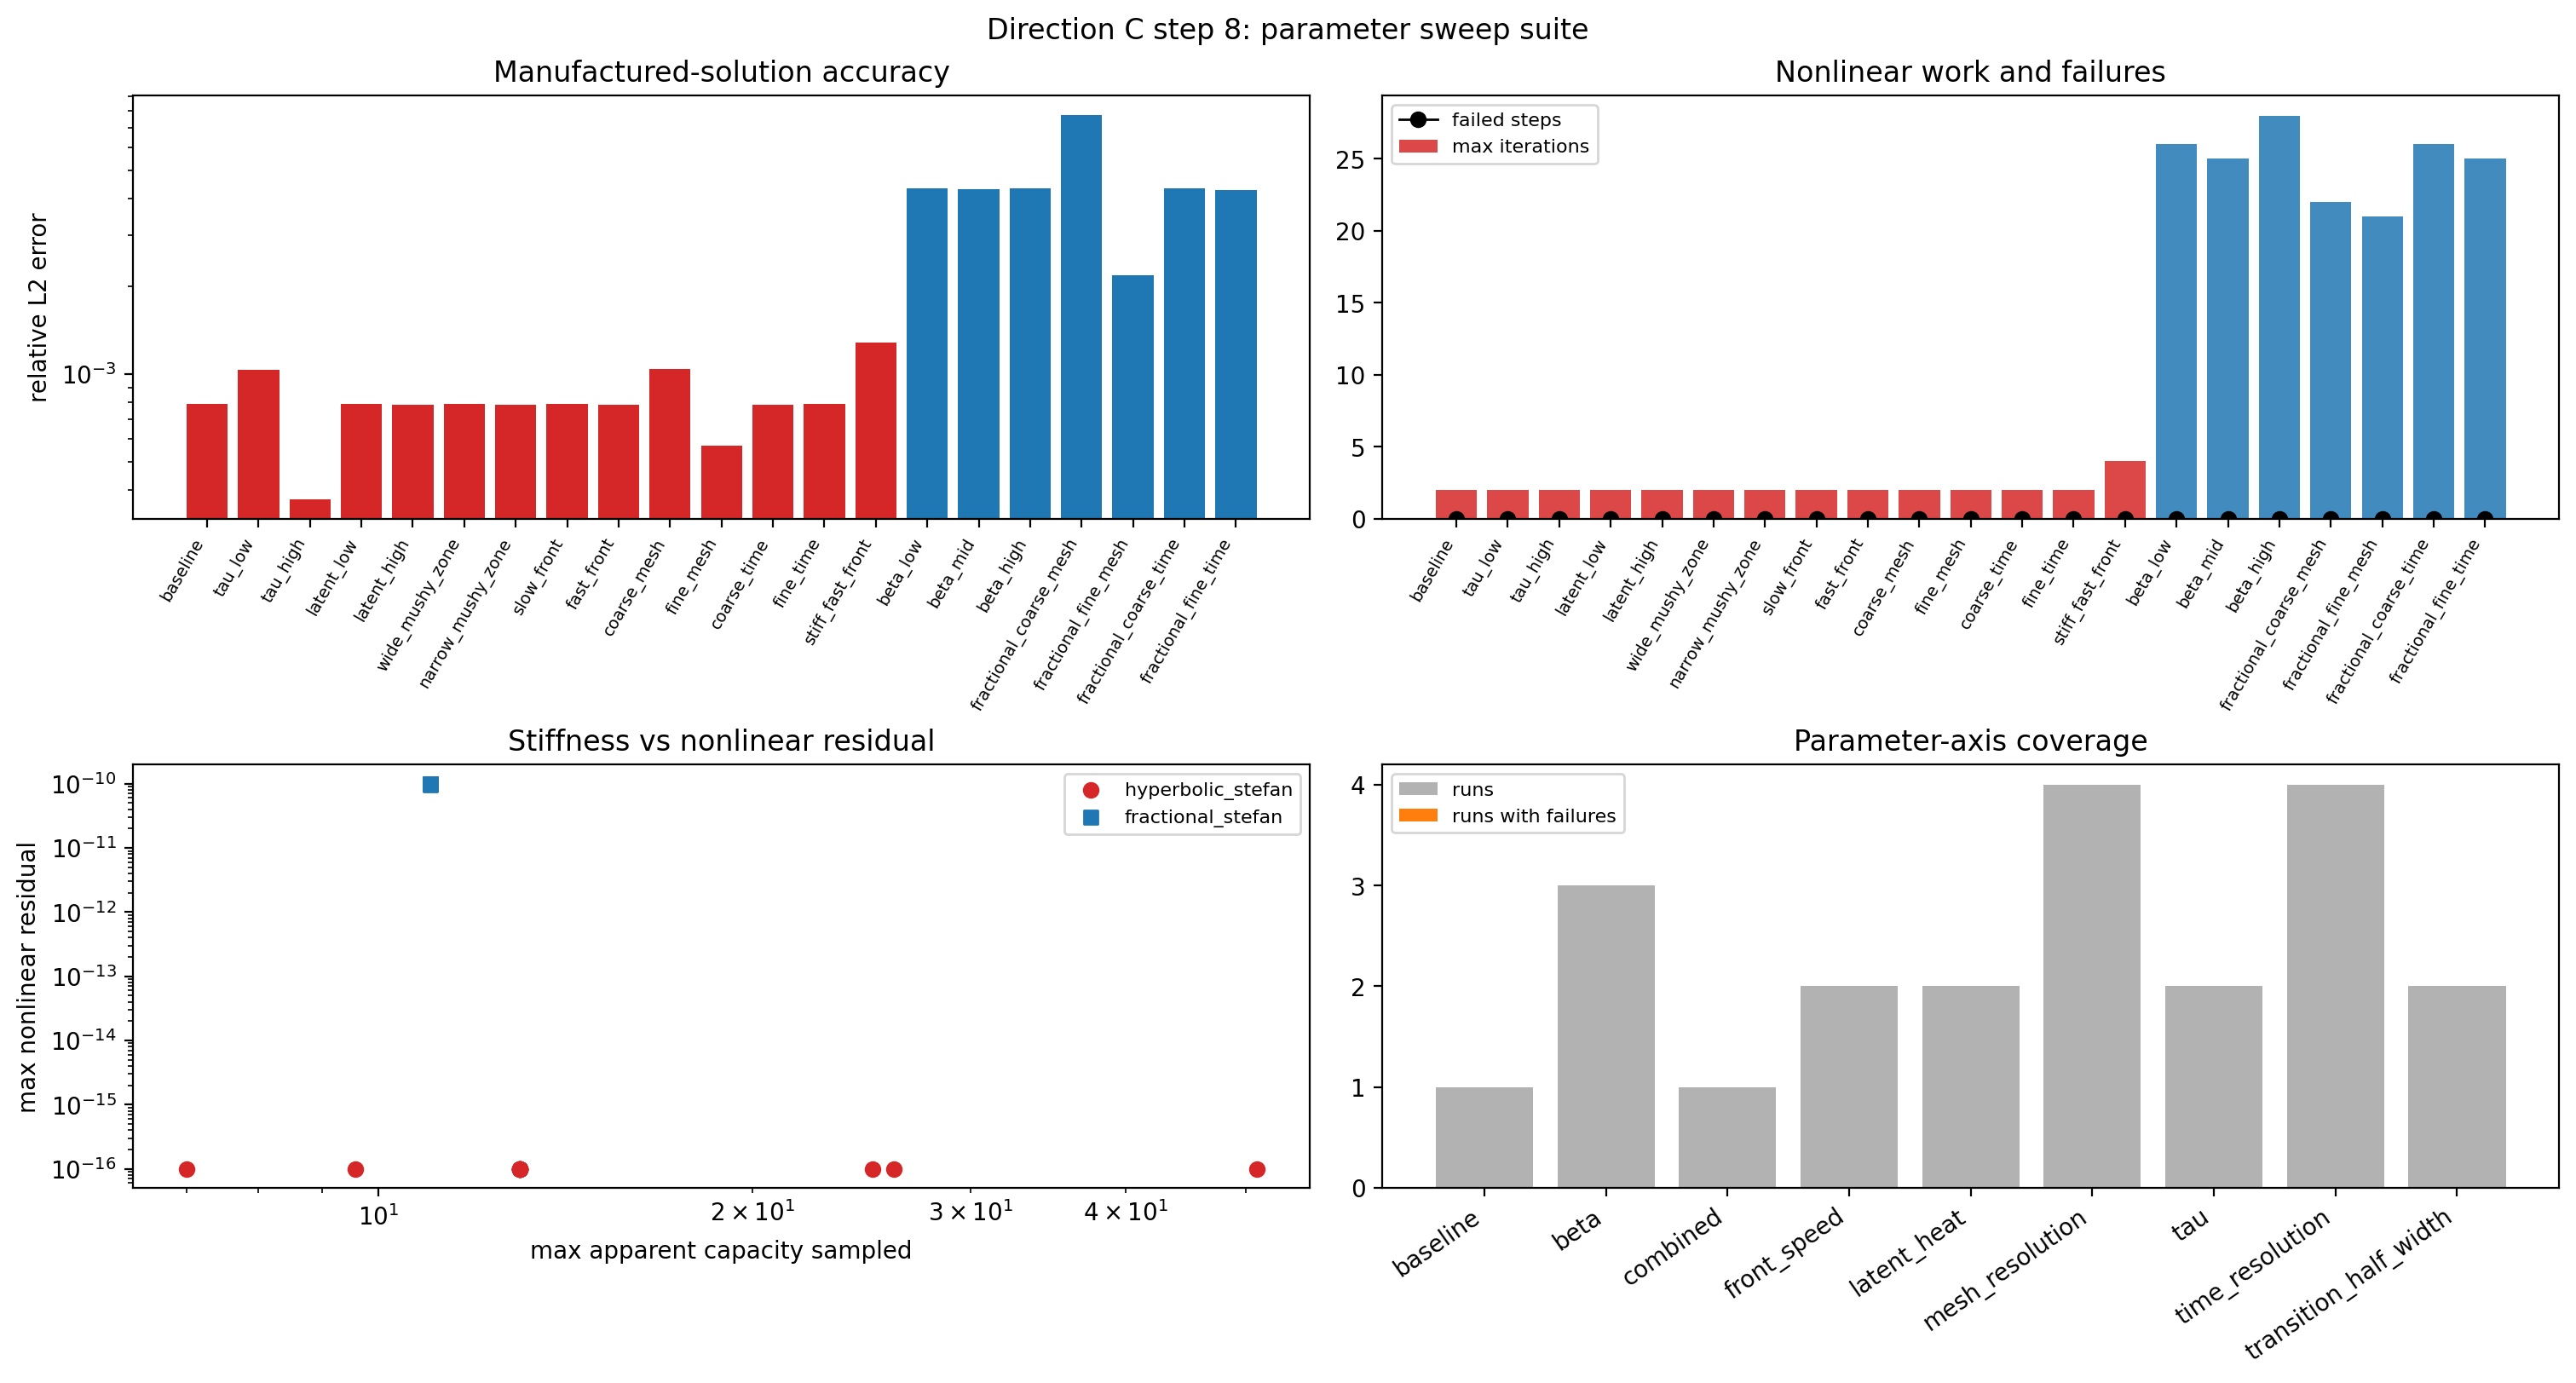
\includegraphics[width=\linewidth]{test_plots/direction_C_nonfourier_phase_change/sweeps/parameter_sweep_suite.png}
  \caption{Direction C parameter-sweep suite. The step-8 matrix collects manufactured errors, nonlinear iteration costs, failed-step counts, stiffness/residual behavior, and coverage by swept parameter axis across hyperbolic and fractional Stefan variants.}
\label{fig:direction-c-parameter-suite}

\end{figure}

\section{Figure Generation Script}

The Direction C report intentionally references existing plot artifacts.  The
helper script
\begin{equation*}
  \texttt{report\_images/generate\_direction\_c\_report\_images.py}
\end{equation*}
therefore checks figure availability and rewrites caption snippets by default,
without rerunning simulations.  From the repository root:
\begin{verbatim}
MPLCONFIGDIR=/tmp/matplotlib \
  /home/user/thermalio/.venv/bin/python \
  report_images/generate_direction_c_report_images.py
\end{verbatim}
To regenerate the underlying application and sweep plots deliberately, pass
\texttt{--regenerate}; add \texttt{--quick} for reduced-size smoke-test
artifacts:
\begin{verbatim}
MPLCONFIGDIR=/tmp/matplotlib \
  /home/user/thermalio/.venv/bin/python \
  report_images/generate_direction_c_report_images.py --regenerate
\end{verbatim}

\appendix

\section{Appendix: Apparent Heat Capacity and Stefan Problems}

The classical Stefan problem is normally written as a heat equation in each
phase plus an interface condition equating latent heat release to conductive
flux imbalance.  Apparent heat capacity avoids explicit interface tracking by
spreading the latent heat over a small temperature band.  The interface becomes
a resolved mushy region, and the heat equation remains a single PDE.  This is
easier to combine with existing finite-volume diffusion operators, but it
introduces a nonlinear and sometimes stiff capacity factor.

\section{Appendix: Why Cattaneo Transport Is Hyperbolic}

Fourier's law sets heat flux instantaneously:
\begin{equation}
  \bm{q} = -k\nabla T.
\end{equation}
Cattaneo's law adds flux relaxation:
\begin{equation}
  \tau_q \partial_t \bm{q} + \bm{q} = -k\nabla T.
\end{equation}
Combining this with energy conservation produces a second time derivative of
temperature.  That second derivative is why the resulting heat equation is
hyperbolic rather than parabolic, and why it has finite thermal-wave speed.

\section{Appendix: Caputo Memory and the L1 Scheme}

The Caputo derivative in \eqref{eq:caputo} weights older temperature changes by
$(t-s)^{-\beta}$.  The singularity near $s=t$ gives strong recent memory, while
the slow power-law decay means old states are never completely forgotten.  The
L1 scheme converts this integral into a history sum over previous time
increments.  For $N$ time steps, a naive implementation stores and sums
$O(N)$ history per step; short-memory truncation reduces that cost by dropping
old increments.

\section{Appendix: Picard Iteration and Anderson Acceleration}

The phase-change solvers are nonlinear because $c_{\mathrm{eff}}$ depends on
temperature.  Picard iteration freezes $c_{\mathrm{eff}}$ at the current
temperature estimate, solves a linear system, then updates the estimate.
Anderson acceleration combines several recent Picard updates to reduce fixed
point error.  In Direction C, the diagnostics report both the iteration count
and residual history, because convergence difficulty is itself a useful
physical/numerical signal when latent heat and mushy-zone width are varied.

\section{Appendix: Reading Energy-Closure Residuals}

The energy residual in \eqref{eq:energy-audit} is not a new PDE variable.  It is
a bookkeeping diagnostic that compares the enthalpy change implied by the final
temperature field with known or inferred energy input.  A small residual
indicates that sensible heat, latent heat, source input, and boundary exchange
are mutually consistent.  A large residual can indicate insufficient
resolution, nonlinear nonconvergence, or a mismatch between the physical
forcing definition and the numerical boundary/source discretization.

\end{document}
